\subsection{Particle phase space}
In the cumulant analysis, measurements are repeated with particles coming from different phase space $(\eta,\phi)$. There are four different $p_\text{T}$ ranges:
\begin{itemize}
\item $0.5<p_\text{T}<5.0$ GeV;
\item $1.0<p_\text{T}<5.0$ GeV;
\item $1.5<p_\text{T}<5.0$ GeV;
\item $2.0<p_\text{T}<5.0$ GeV;
\end{itemize}
While calculating the $2k$-particle correlations, all the $2k$ particles will come from the same $p_\text{T}$ window. Note it is different from traditional differential cumulant measurements, where only one out of $2k$ particles comes from the assigned $p_\text{T}$ range. The traditional differential cumulant measurement assumes that the flow in different $p_\text{T}$ ranges share the same event plane, however, measurement of flow decorrelation in $p_\text{T}$ shows that such assumption is ungrounded. In this analysis, all the particles are coming from the same $p_\text{T}$ range, which also simplifies the differential cumulant formula, without special treatment of reference particles.

\begin{figure}[H]
\centering
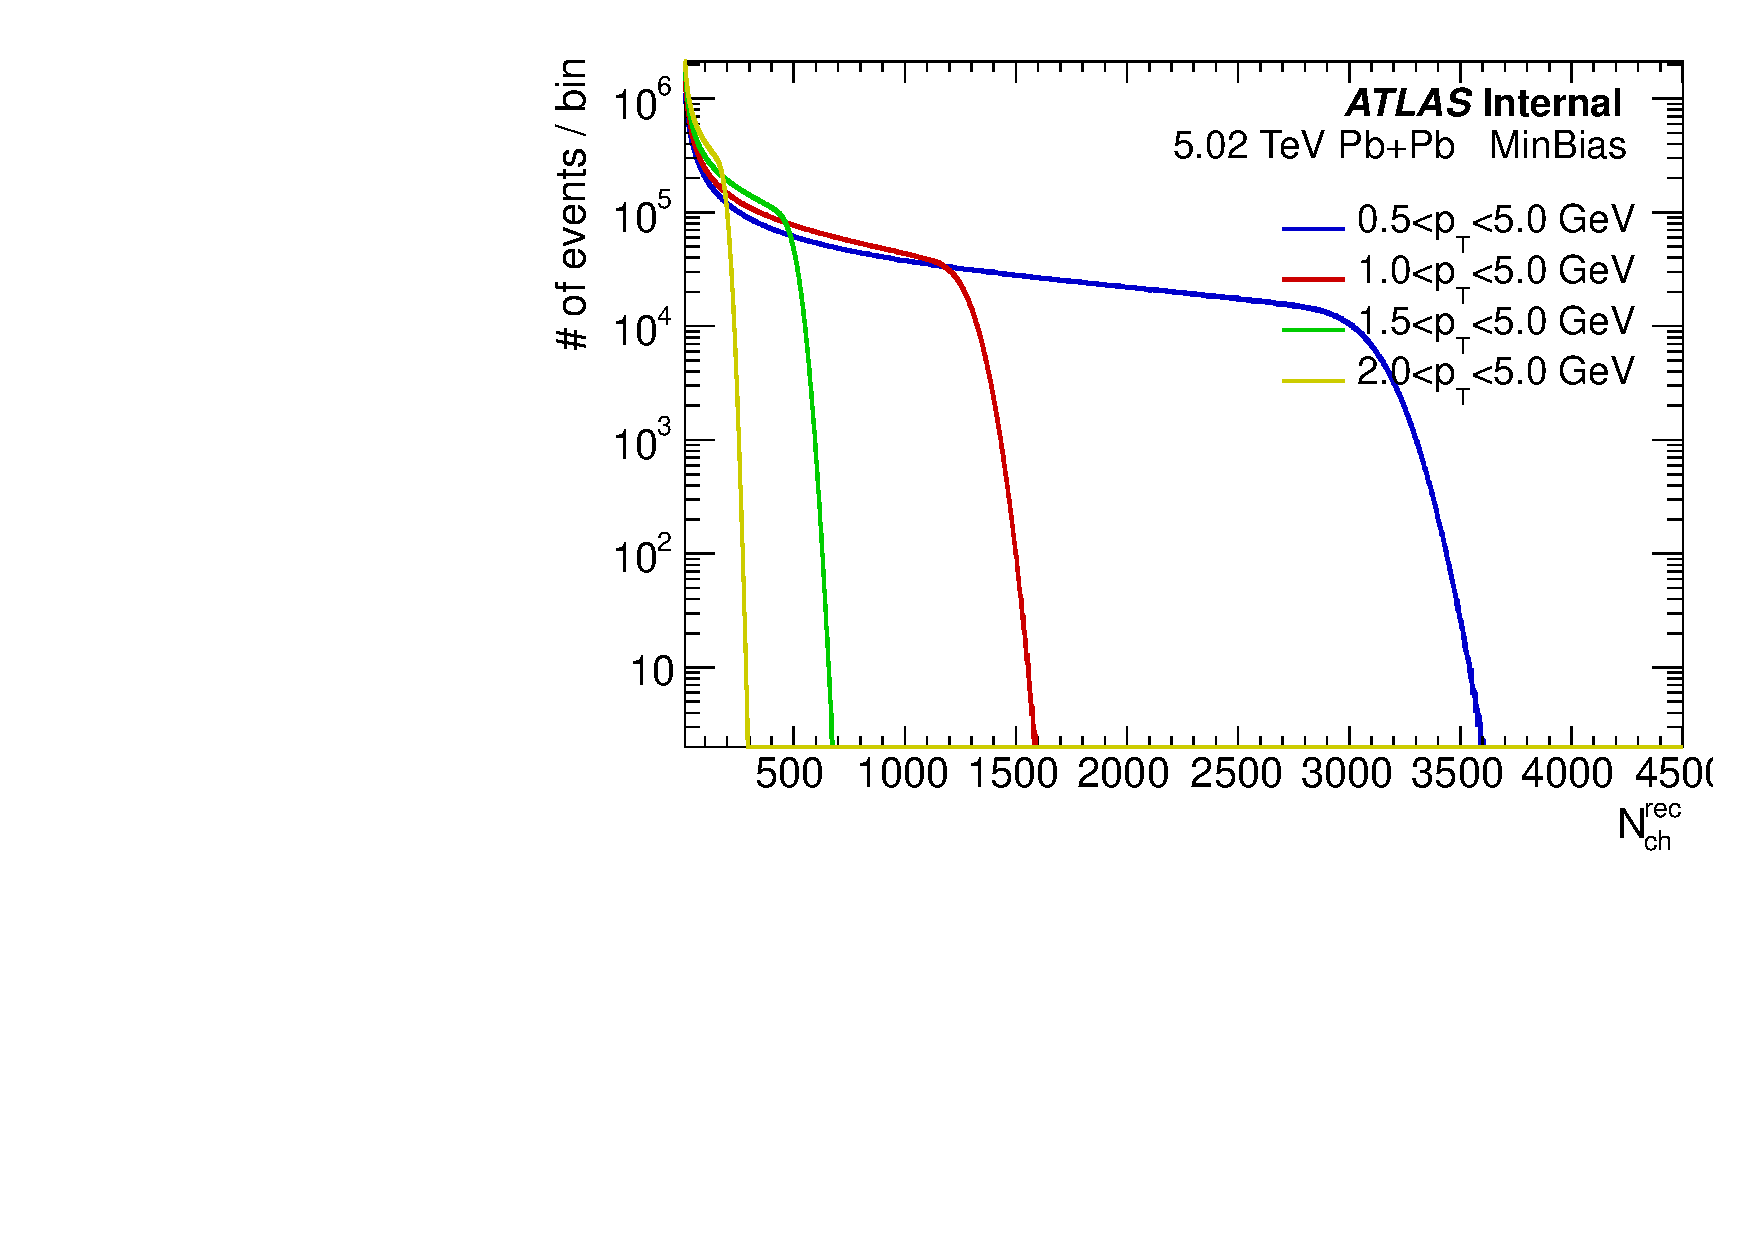
\includegraphics[width=.75\linewidth]{figs/sec_ana/cumuPhase_nTrkPt.pdf}
\caption{Distribution of reconstructed tracks from different $p_\text{T}$ ranges.}
\label{fig:cumuAna_PHASE_pt}
\end{figure}
To get an idea of how many particles are included with different $p_\text{T}$ cuts, Fig.~\ref{fig:cumuAna_PHASE_pt} shows the distributions of reconstructed tracks $N_{ch}^{rec}$ from different $p_\text{T}$ ranges. For $0.5<p_\text{T}<5.0$ GeV, the $N_{ch}^{rec}$ extends to 3600, while for the highest $p_\text{T}$ cut $2.0<p_\text{T}<5.0$ GeV, the largest $N_{ch}^{rec}$ is less than 300. This means that the statistical errors for the highest $p_\text{T}$ cut will be quite large.

In the standard cumulant method, all the particles have $-2.5<\eta<2.5$, while in the subevent method, the subevent is defined based on $\eta$:
\begin{itemize}
\item Subevent $a$: particles from $-2.5/3<\eta<2.5/3$;
\item Subevent $b$: particles from $-2.5<\eta<-2.5/3$;
\item Subevent $c$: particles from $2.5/3<\eta<2.5$;
\end{itemize}
where additional $\eta$ gaps can be applied between subevent $a$ and $b(c)$ to further suppress the long-range non-flow correlations.

\begin{figure}[H]
\centering
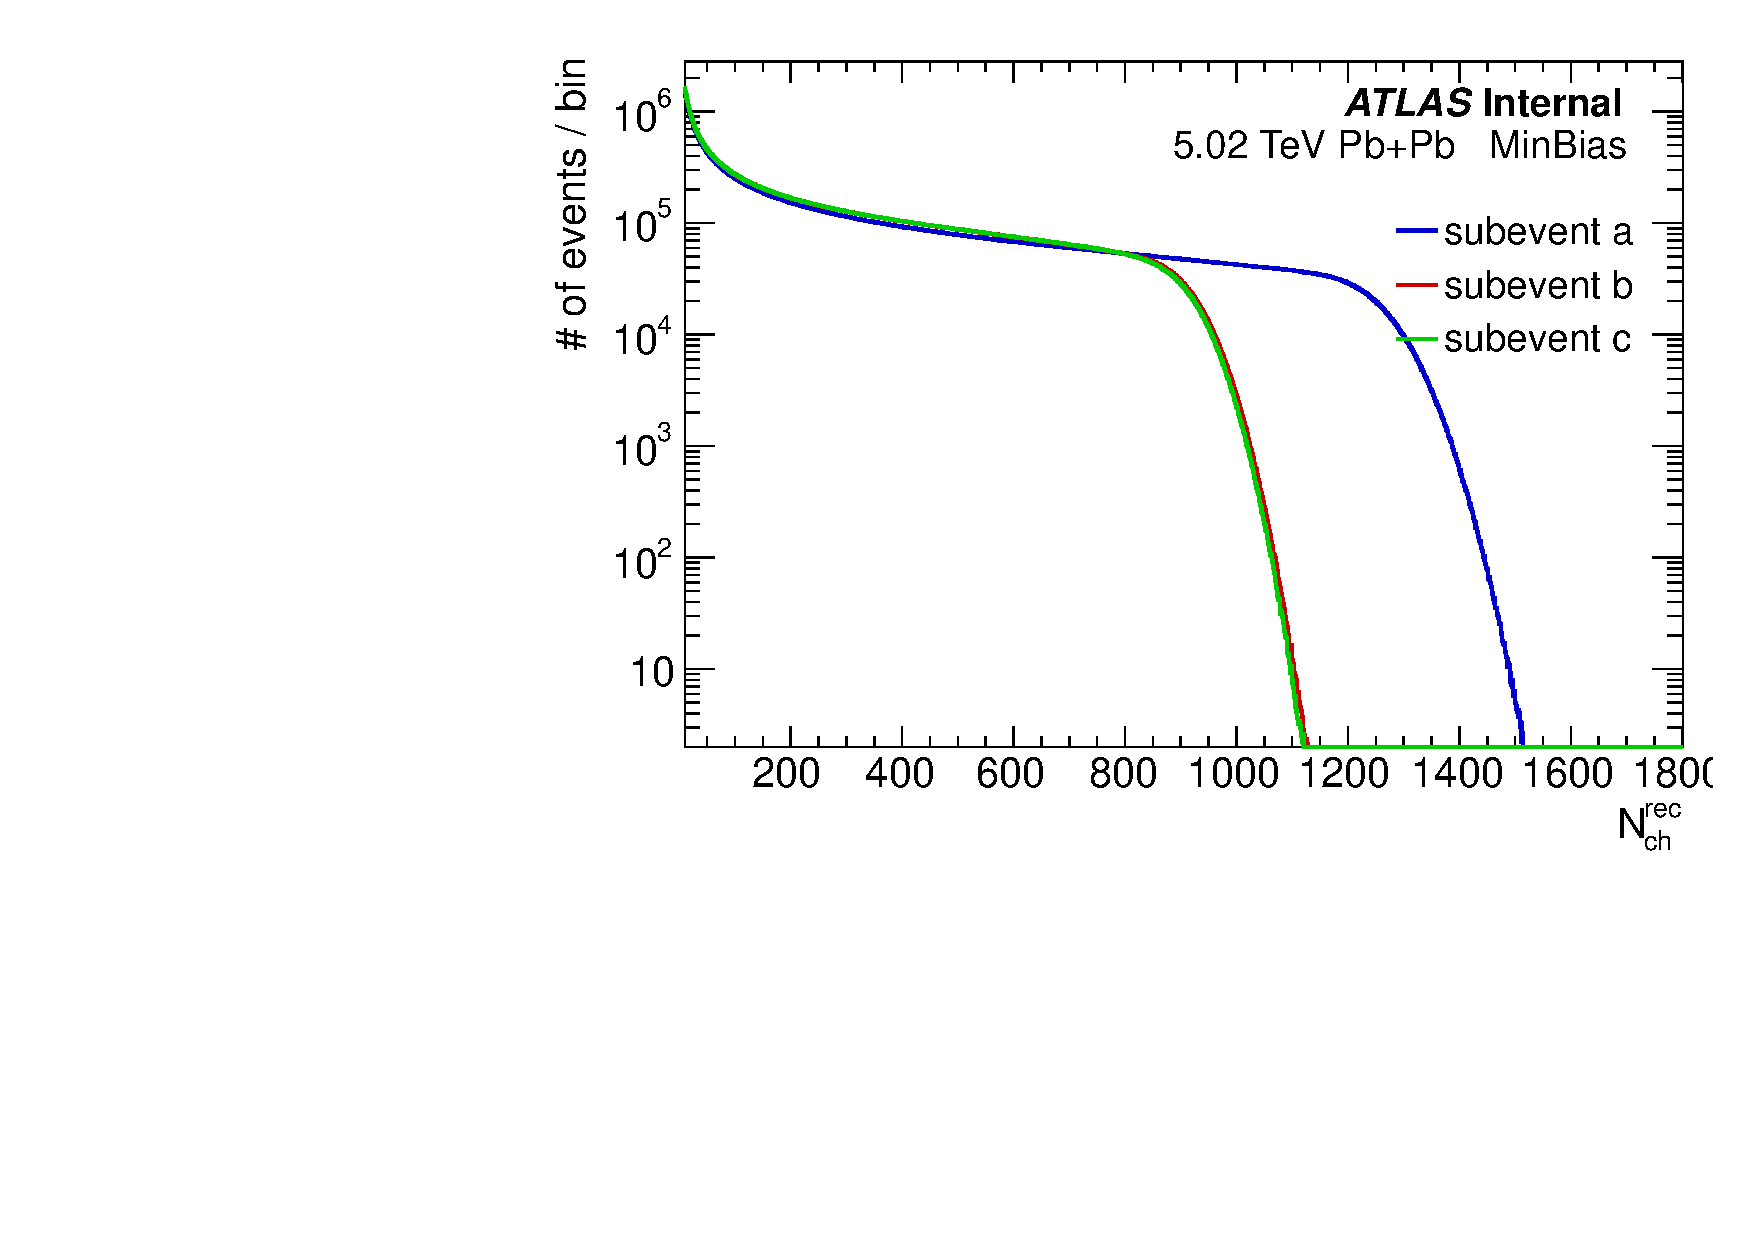
\includegraphics[width=.75\linewidth]{figs/sec_ana/cumuPhase_nTrkSub.pdf}
\caption{Distribution of reconstructed tracks from different $\eta$ ranges (subevents).}
\label{fig:cumuAna_PHASE_sub}
\end{figure}
Fig.~\ref{fig:cumuAna_PHASE_sub} shows the distribution of reconstructed tracks from different $\eta$ ranges, which are defined as subevent $a$, $b$ and $c$. $N_{ch}^{rec}$ is largest in subevent $a$ with $-2.5/3<\eta<2.5/3$, mainly due to two reasons: truth $N_{ch}$ slightly decreases as $|\eta|$ grows and the tracking efficiency also decrease at large $|\eta|$. Meanwhile, $N_{ch}^{rec}$ from subevent $b$ and $c$ are slightly different, which originates from the facts that: $1)$ mean of $z$ position of primary vertex is slightly shifted to the negative side, $2)$ tracking efficiency is not symmetric between positive and negative $\eta$.



\subsection{Trigger weighting}
Events in this analysis are collected by two minimum bias triggers and multiple UCC triggers. The statistics of collected events are shown in the left panel of Fig.~\ref{fig:ana_evtWght}, where the UCC triggers greatly enhanced the statistics in the region of FCal $E_\text{T}>4.2$ TeV. However, such enhancement will introduce potential bias when calculating cumulants in the event class defined by $N_{ch}^{rec}$. 

\begin{figure}[H]
\centering
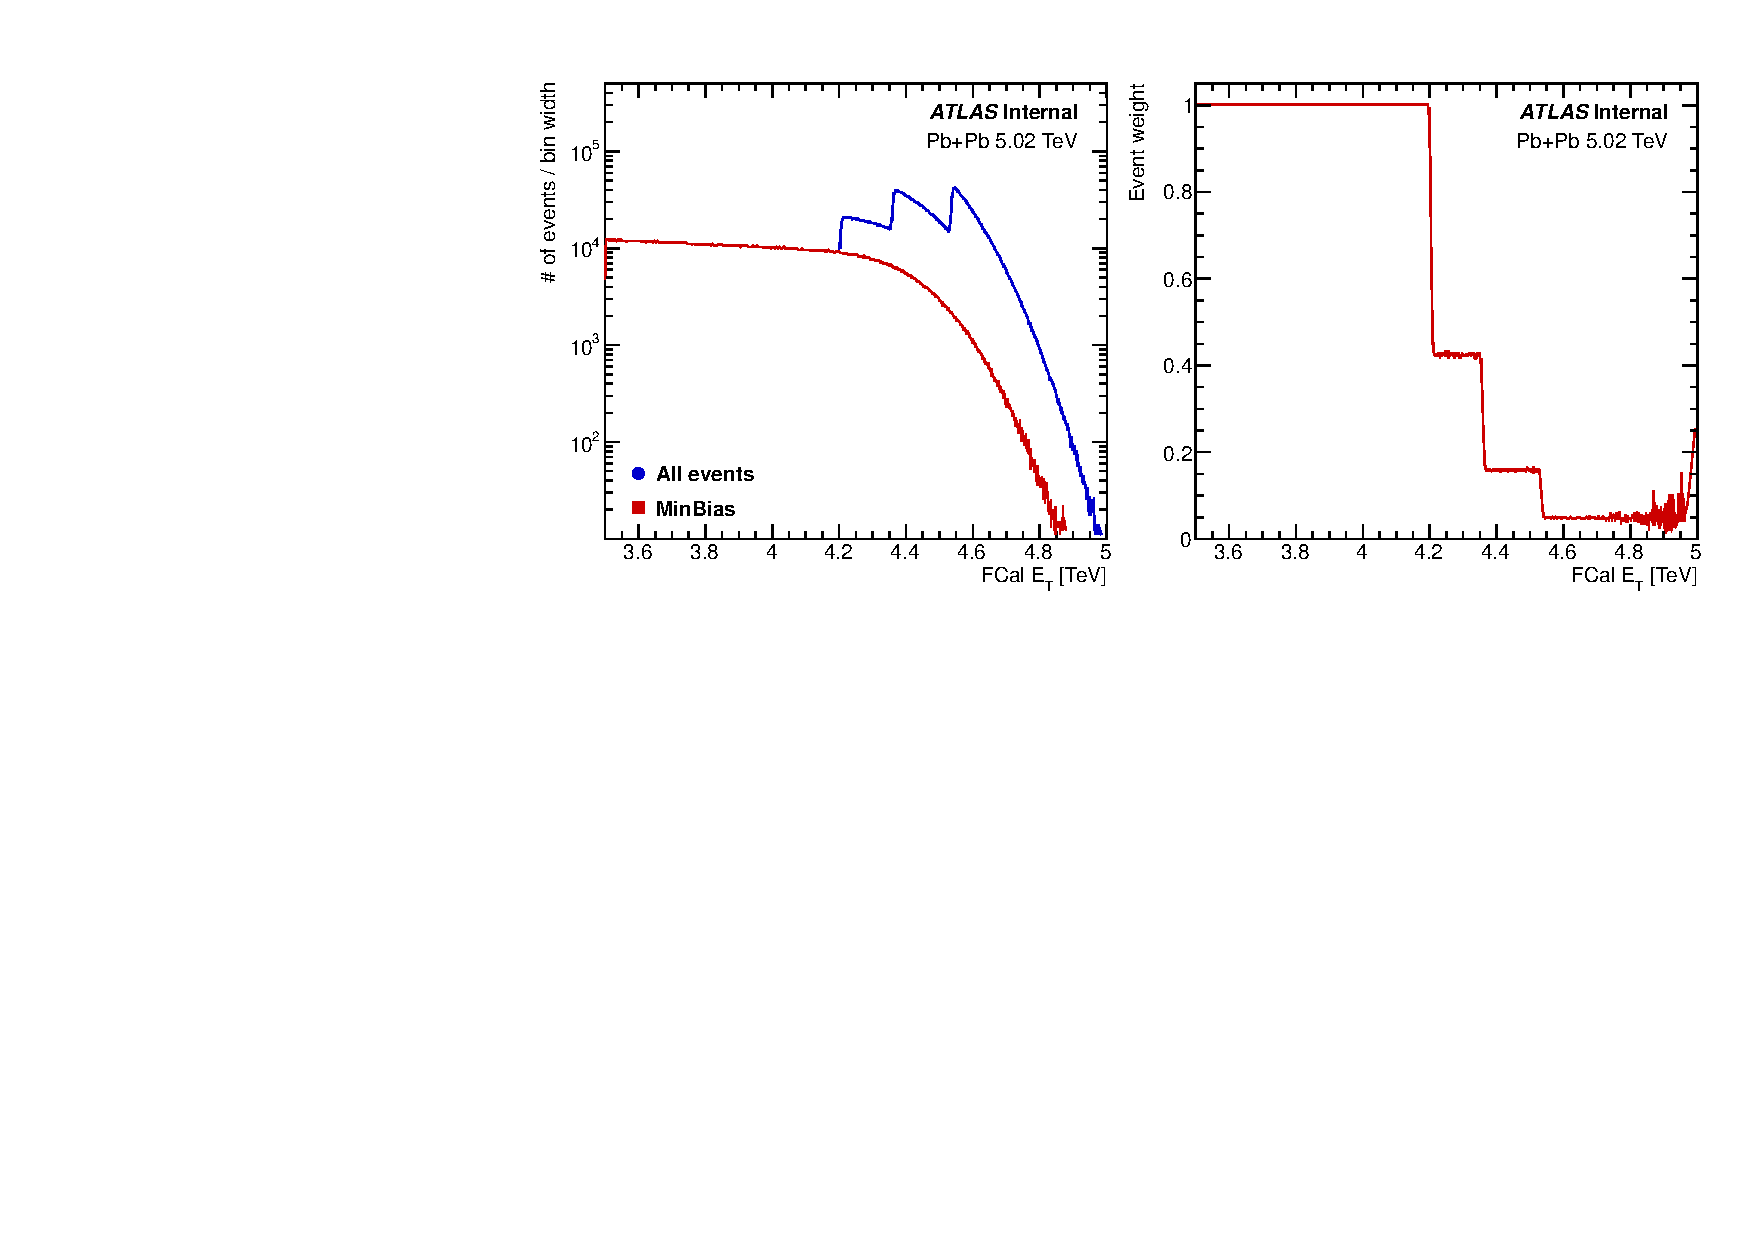
\includegraphics[width=.9\linewidth]{figs/sec_ana/trig_weight.pdf}
\caption{Additional event weights applied in order to properly include the UCC events.}
\label{fig:ana_evtWght}
\end{figure}

To properly include the events that passed UCC trigger, an event weight $w_{trig}$ has been applied to the $\lr{corr_{n}\{2k\}}$ calculation:
\begin{equation}
w_{trig}\equiv \frac{\text{events passed MinBias}}{\text{event passed MinBias and UCC}}
\end{equation}
where $w_{trig}$ is only estimated as a function of FCal $E_\text{T}$, as shown in the right panel of Fig.~\ref{fig:ana_evtWght}. $w_{trig}$ equals 1 for minimum-bias events and it lowers to three steps as FCal $E_\text{T}$ increases.

\begin{figure}[H]
\centering
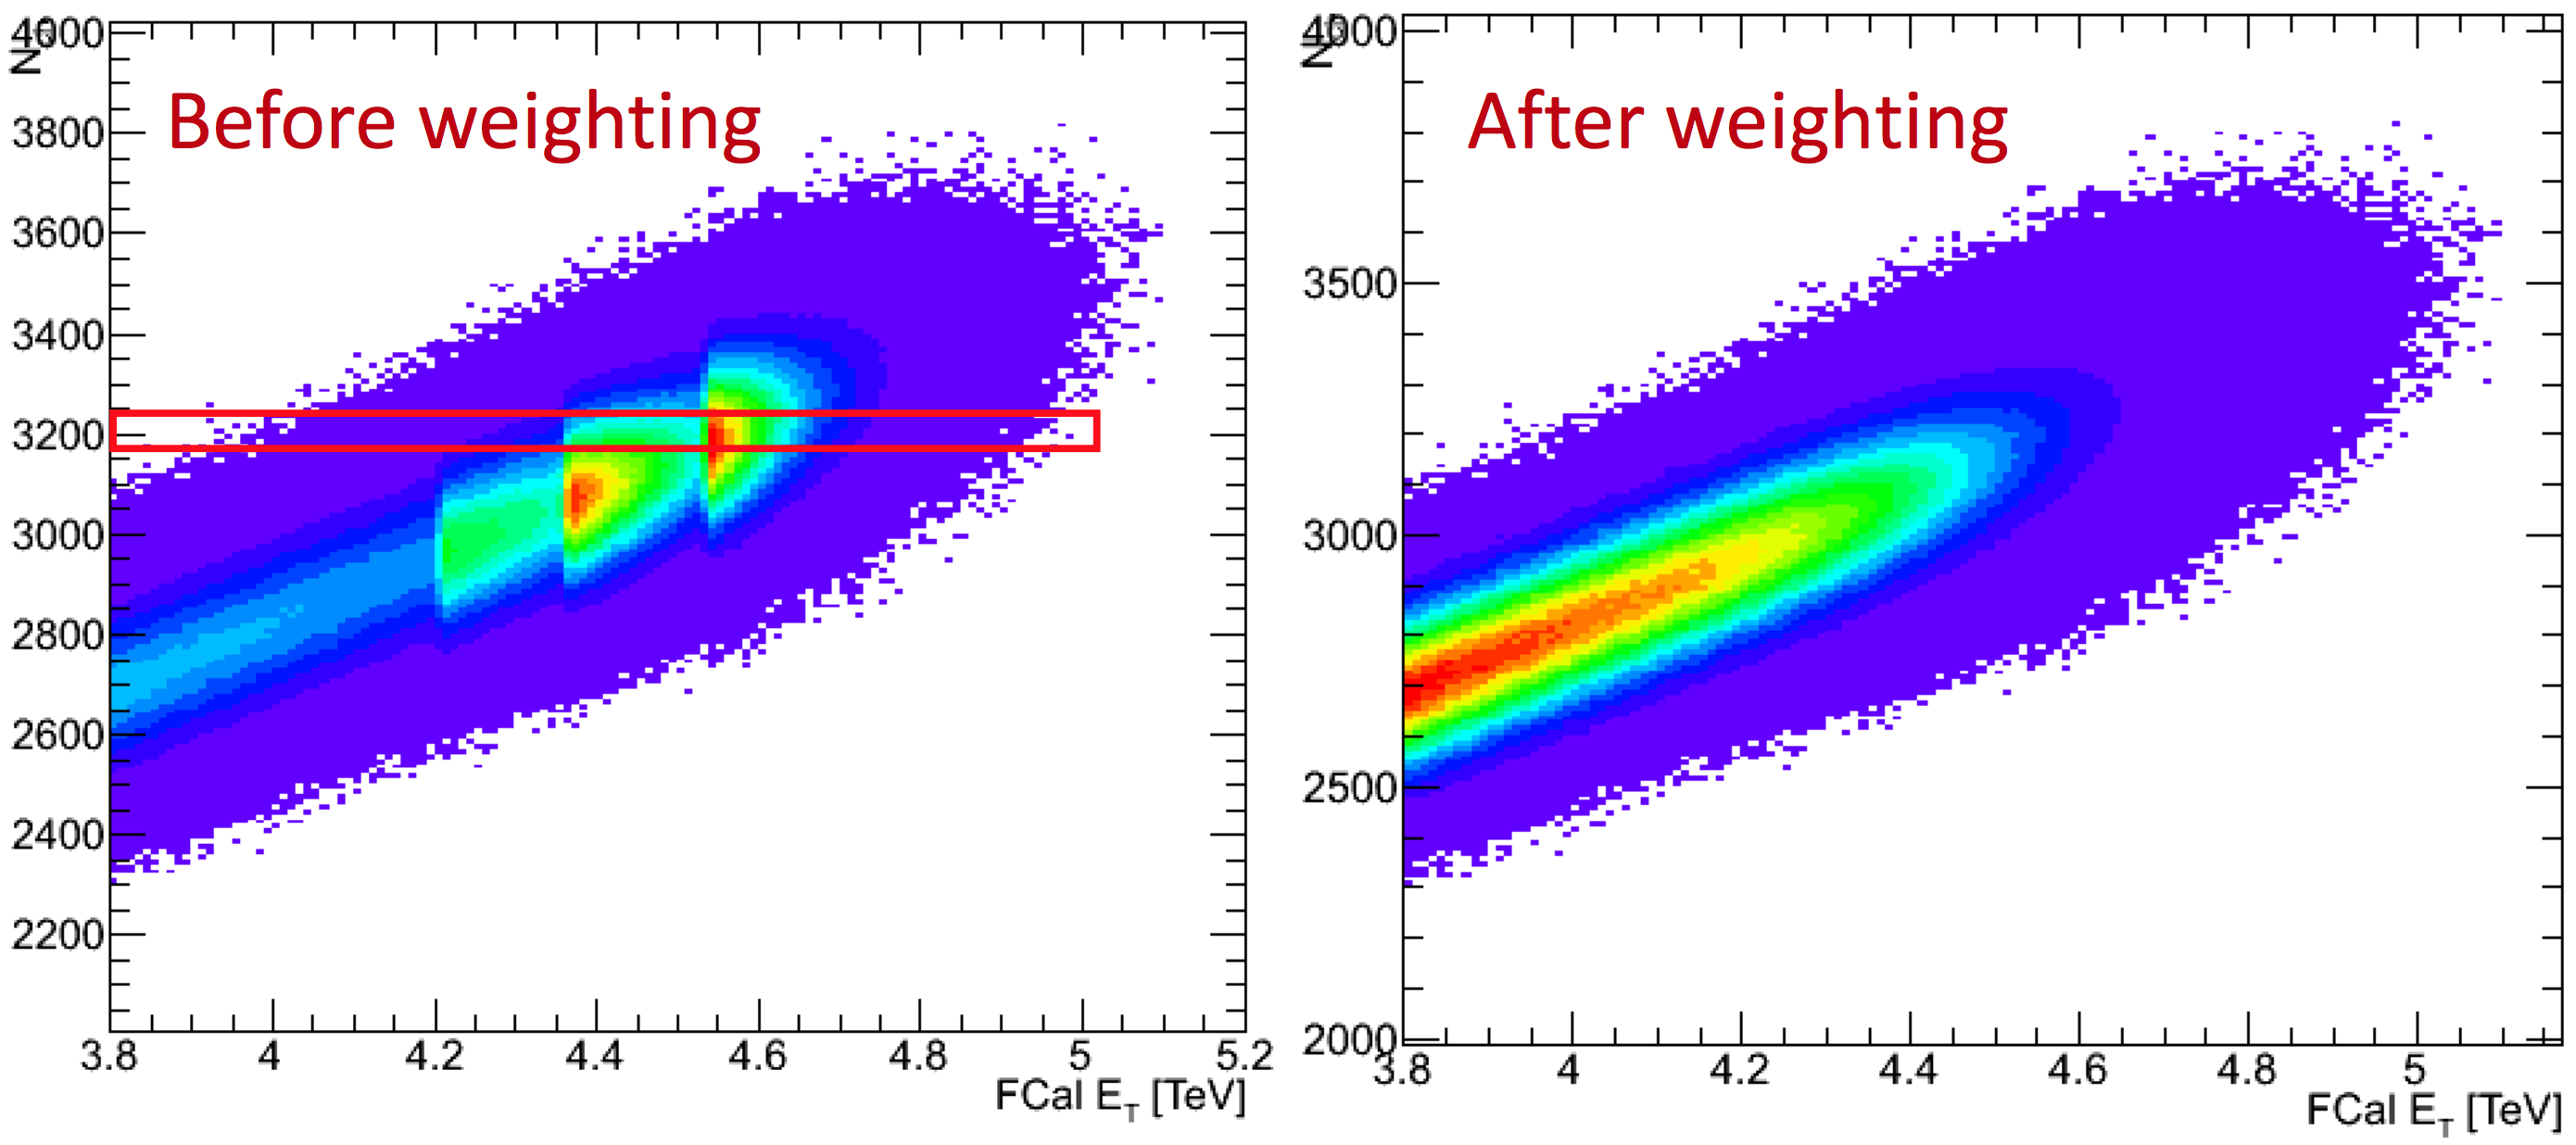
\includegraphics[width=.9\linewidth]{figs/sec_ana/evtWeight_comp.png}
\caption{Correlation between FCal sum $E_T$ and reconstructed tracks $N_{ch}^{rec}$, before (left) and after (right) applying the UCC trigger weights.}
\label{fig:ana_evtWght_comp}
\end{figure}
As one demonstration of how this event weight works, the correlation between FCal $E_\text{T}$ and number of reconstructed tracks $N_{ch}^{rec}$ is shown in Fig.~\ref{fig:ana_evtWght_comp}. Before $w_{trig}$ is applied, enhancement of statistics is observed in the large FCal $E_\text{T}$ region, while after applying $w_{trig}$, the minimum-bias + UCC distribution behaves just like the minimum-bias events as expected.



\subsection{Flattening procedure}
In heavy ion collisions, since the event plane angle fluctuates randomly event-by-event, the particle $\phi$ angle distribution averaged over many events should be flat, and the discrepancy is denoted as the detector effects. From the Monte-Carlo sample, tracking efficiency and fakes can be estimated as a function of $\eta$ and $p_\text{T}$, but the residual detector effects in the $\phi$ plane needs further correction, and the procedure is named as "flattening".

\begin{figure}[H]
\centering
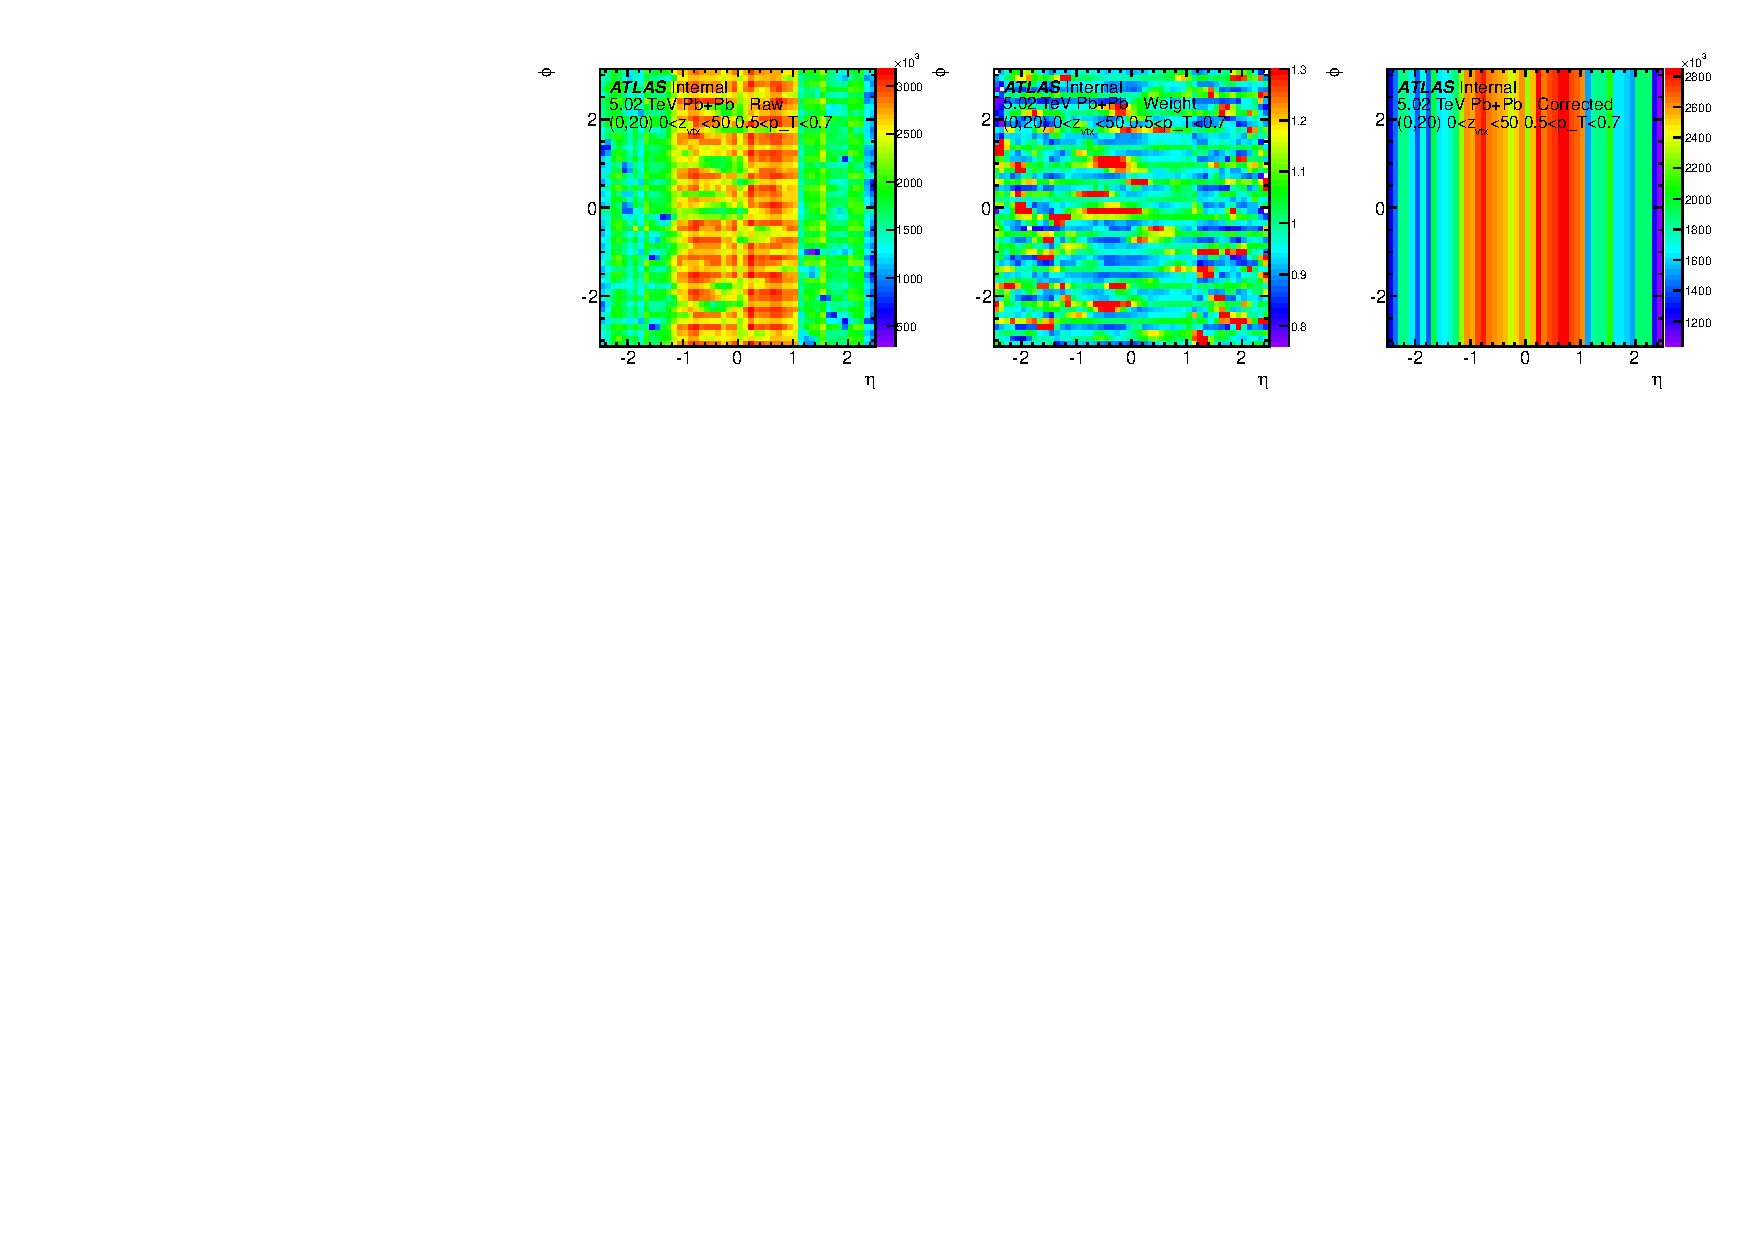
\includegraphics[width=.9\linewidth]{figs/sec_ana/cumuFlat_Cent0_Zvtx5_Chg0_Pt1.pdf}
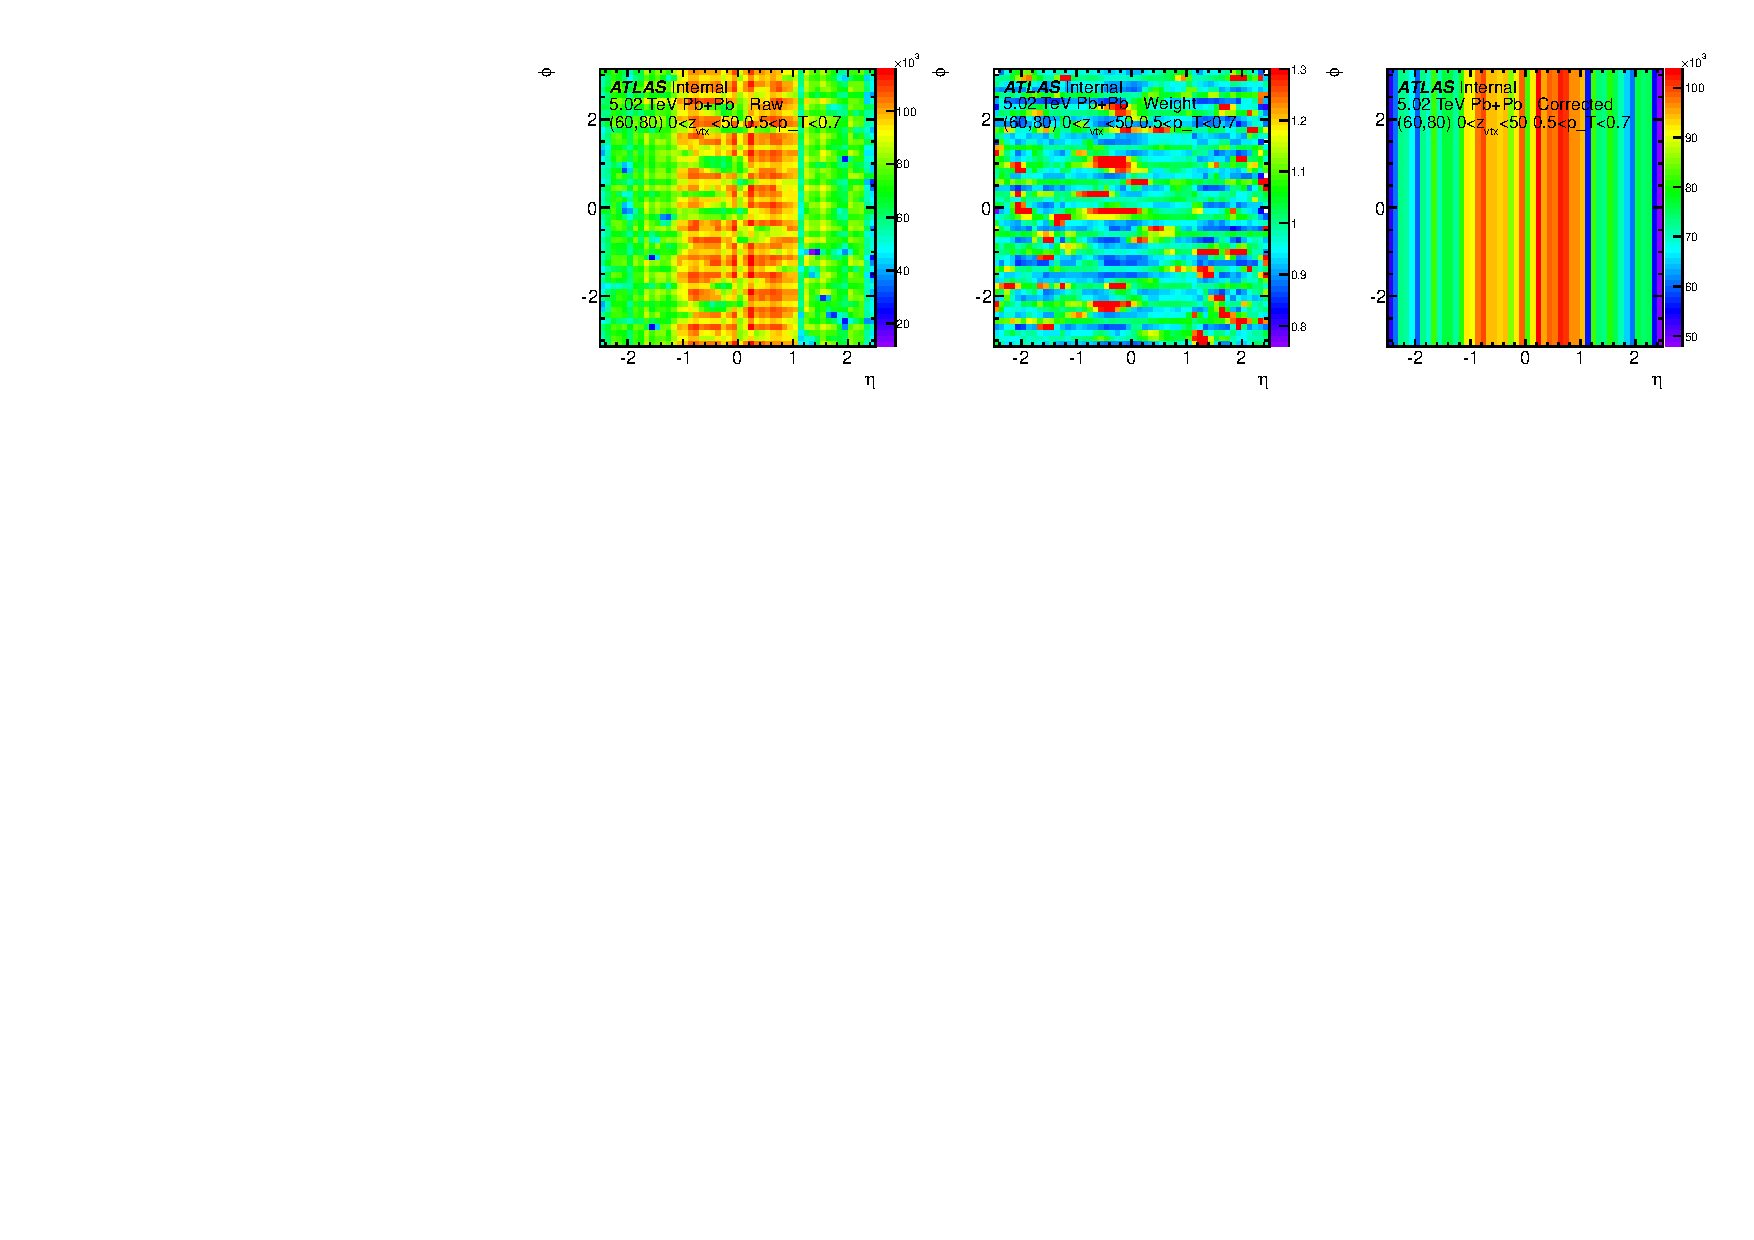
\includegraphics[width=.9\linewidth]{figs/sec_ana/cumuFlat_Cent3_Zvtx5_Chg0_Pt1.pdf}
\caption{Demonstration of flattening procedure in different centralities: top row is $0-20\%$ and bottom row is $60-80\%$. Left column are the raw $(\eta,\phi)$ distributions, middle column are the estimated correction factor $w_{\phi}$, right column are the corrected $(\eta,\phi)$ distributions. }
\label{fig:cumuAna_FLAT_Cent}
\end{figure}
Left column of Fig.~\ref{fig:cumuAna_FLAT_Cent} shows the raw $(\eta,\phi)$ distribution without any correction, and several "holes" are clearly observed in the transverse plane. In order to correct this detector effect, the correction factor $w_\phi$ is defined as:
\begin{equation}
w_\phi(\eta,\phi)\equiv\frac{\lr{N(\delta\eta)}}{N(\delta\eta,\delta\phi)}
\end{equation}
where $N(\delta\eta,\delta\phi)$ is the number of particles in the small $(\eta,\phi)$ phase-space window; and $\lr{N(\delta\eta)}$ is the mean number of particles in the small $\eta$ window averaged over the whole $\phi$ range. The middle panel gives an example of the $w_\phi(\eta,\phi)$: for the "holes" in raw $(\eta,\phi)$ distributions, $w_\phi$ is larger than 1. Right column shows the $(\eta,\phi)$ distribution after the correction, and as expected, for each narrow $\eta$ slice, the corrected $\phi$ distribution is uniform. This correction $w_{\phi}$ will be applied as the particle weight when calculating the $\lr{corr_{n}\{2k\}}$.

Since the detector effect depends on the occupancy of the detector, $w_\phi$ is evaluated in different centrality ranges. Fig.~\ref{fig:cumuAna_FLAT_Cent} shows a comparison between centrality $0-20\%$ and $60-80\%$. The correction factors are not identical, but very similar between the two centralities.

\begin{figure}[H]
\centering
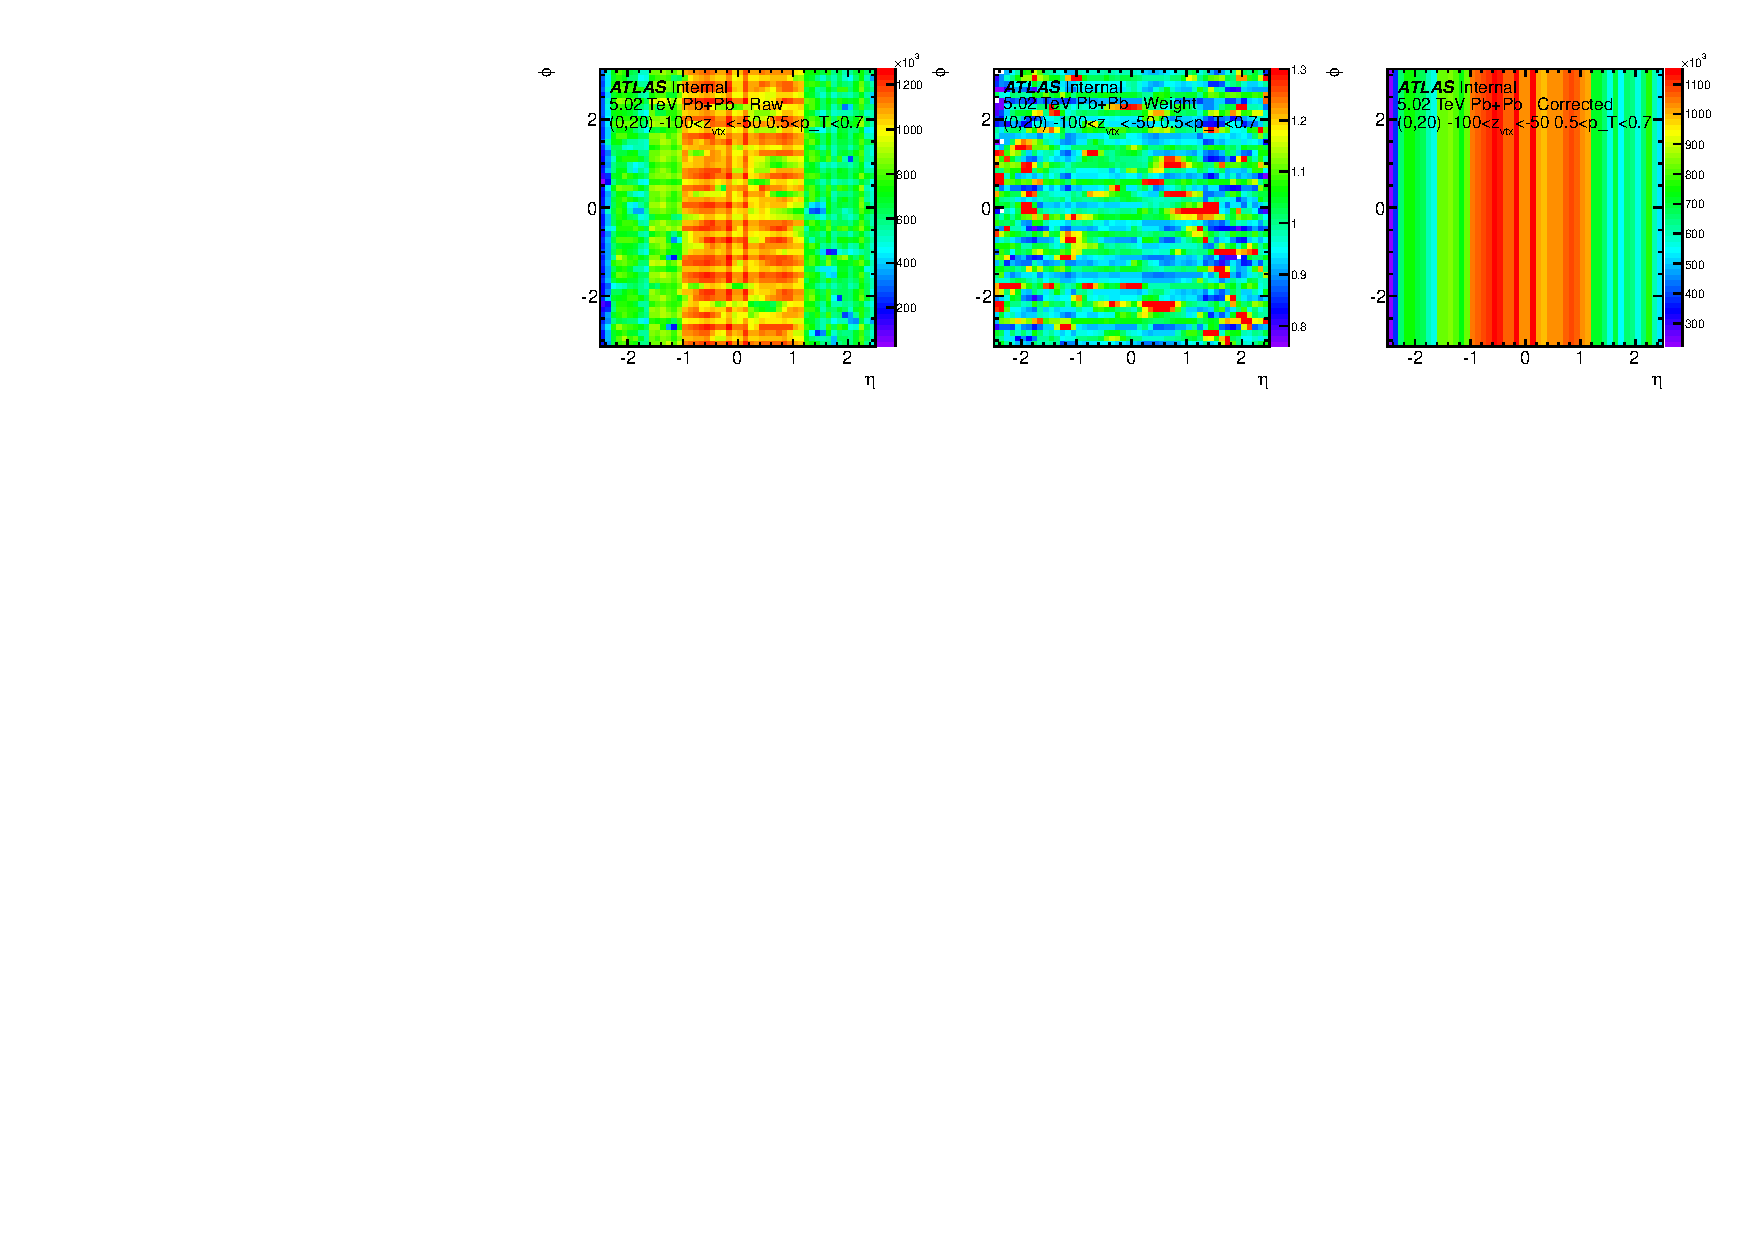
\includegraphics[width=.9\linewidth]{figs/sec_ana/cumuFlat_Cent0_Zvtx3_Chg0_Pt1.pdf}
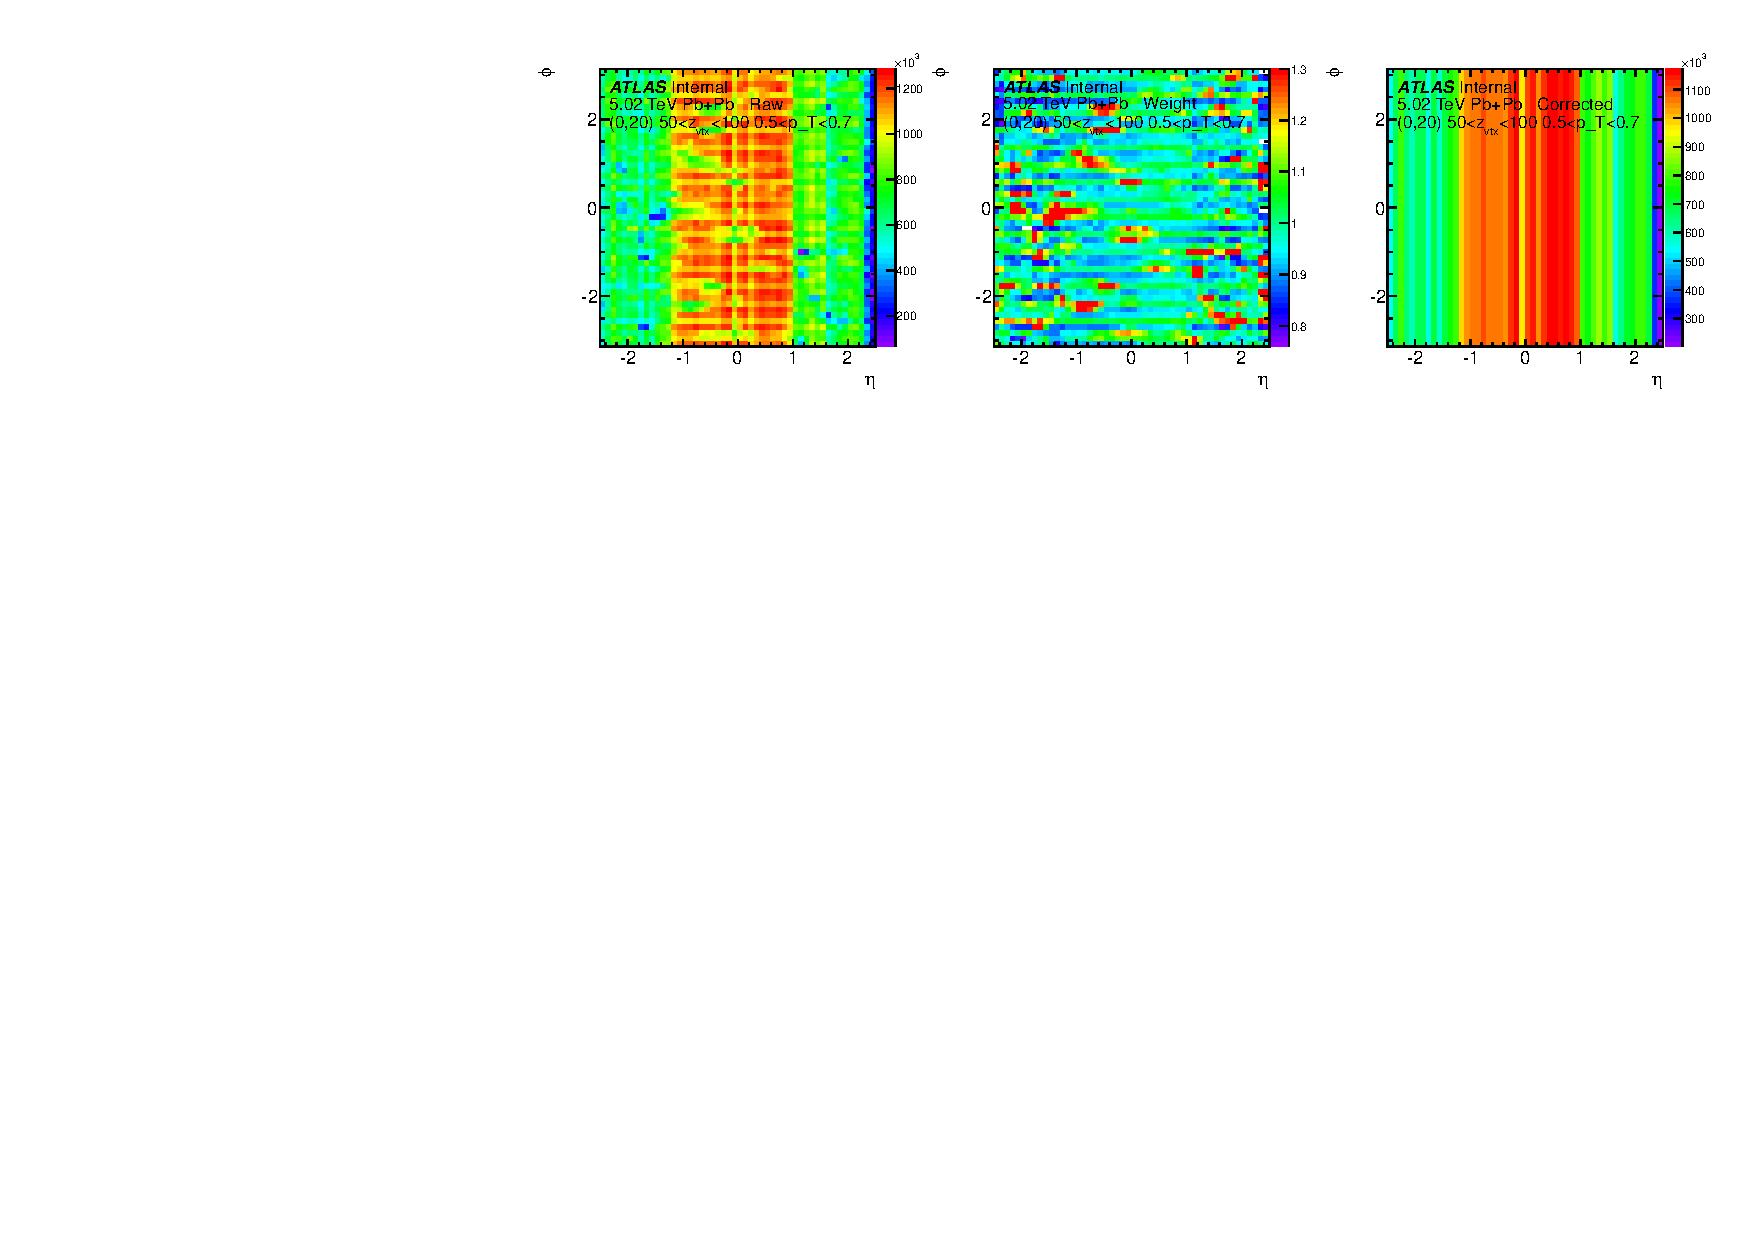
\includegraphics[width=.9\linewidth]{figs/sec_ana/cumuFlat_Cent0_Zvtx6_Chg0_Pt1.pdf}
\caption{Demonstration of flattening procedure in different $z_{vtx}$ ranges: top row is from -100 mm$<z_{vtx}<$-50 mm and bottom row is from 50 mm$<z_{vtx}<$100 mm. Left column are the raw $(\eta,\phi)$ distributions, middle column are the estimated correction factor $w_{\phi}$, right column are the corrected $(\eta,\phi)$ distributions.}
\label{fig:cumuAna_FLAT_Zvtx}
\end{figure}

\begin{figure}[H]
\centering
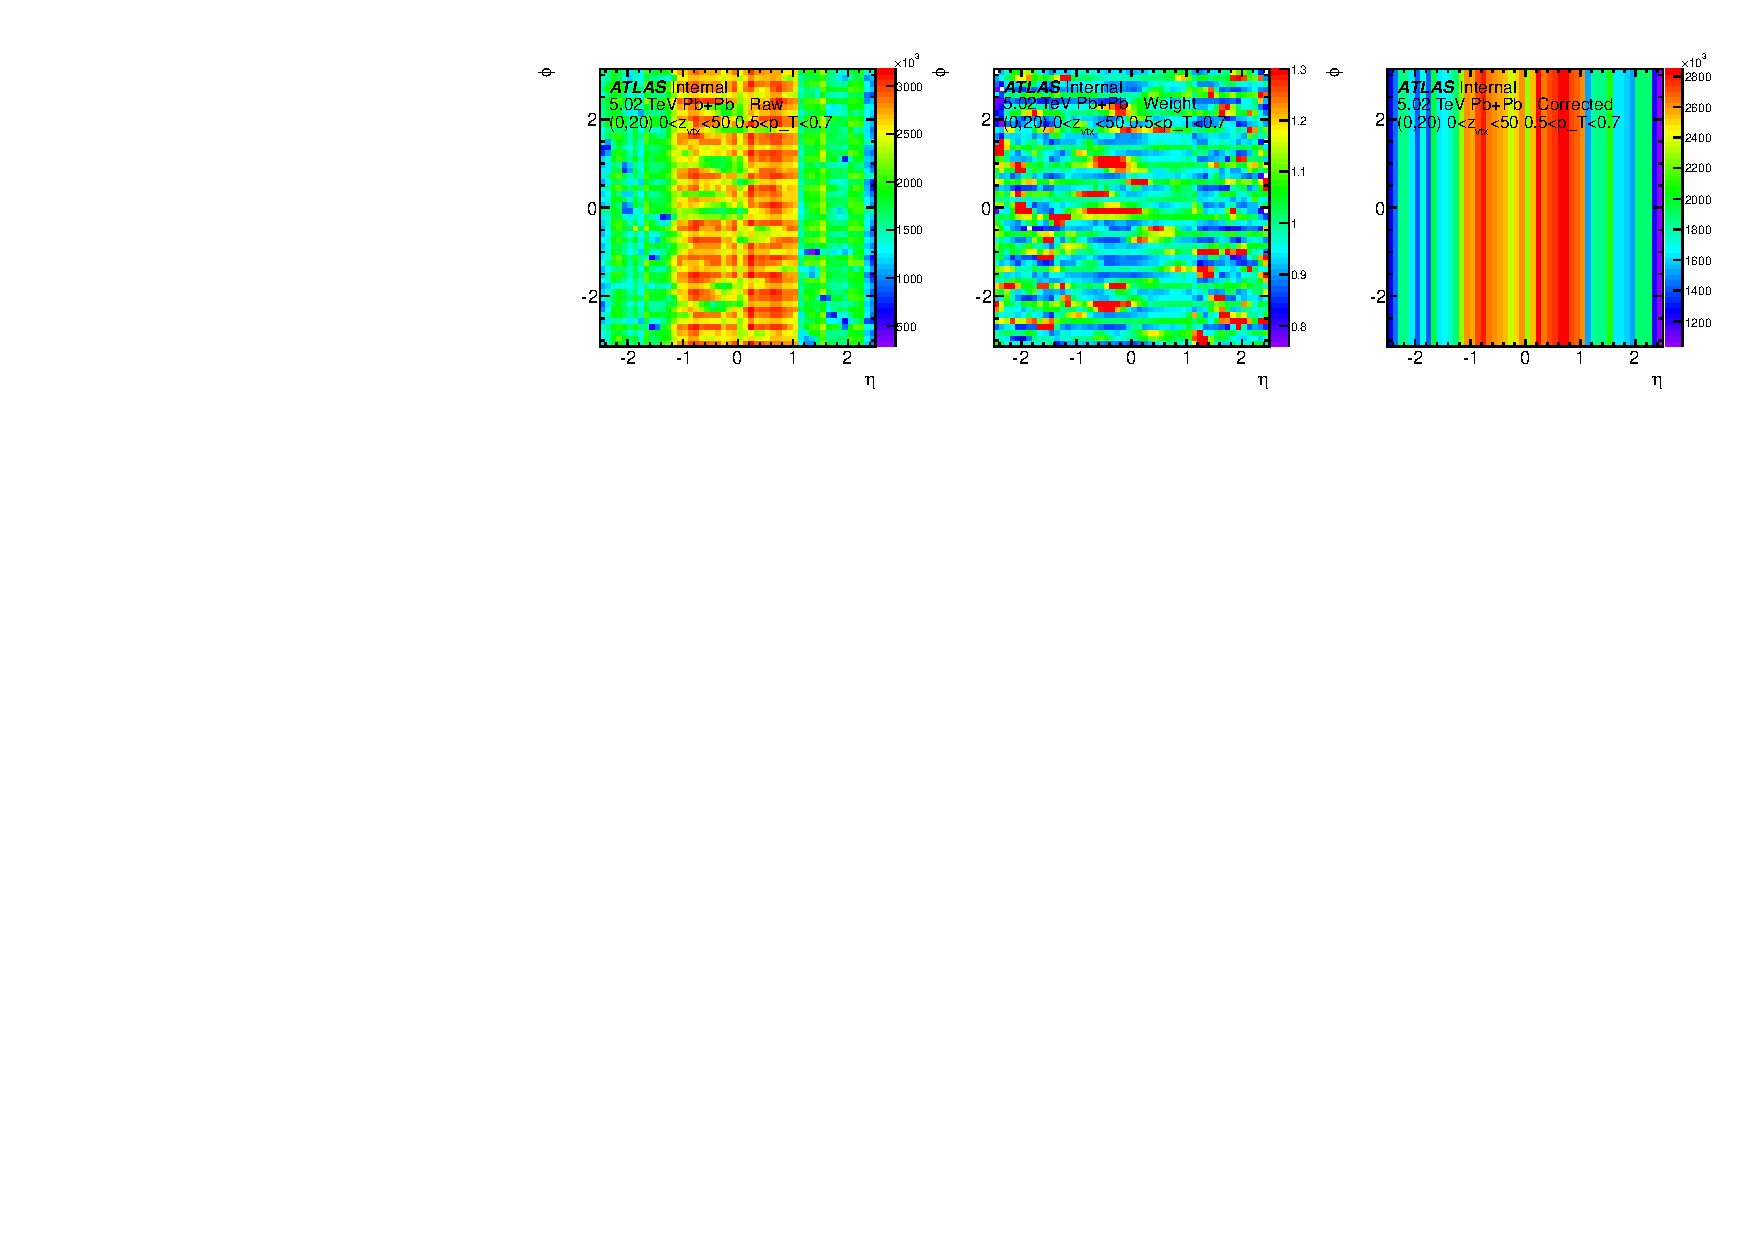
\includegraphics[width=.9\linewidth]{figs/sec_ana/cumuFlat_Cent0_Zvtx5_Chg0_Pt1.pdf}
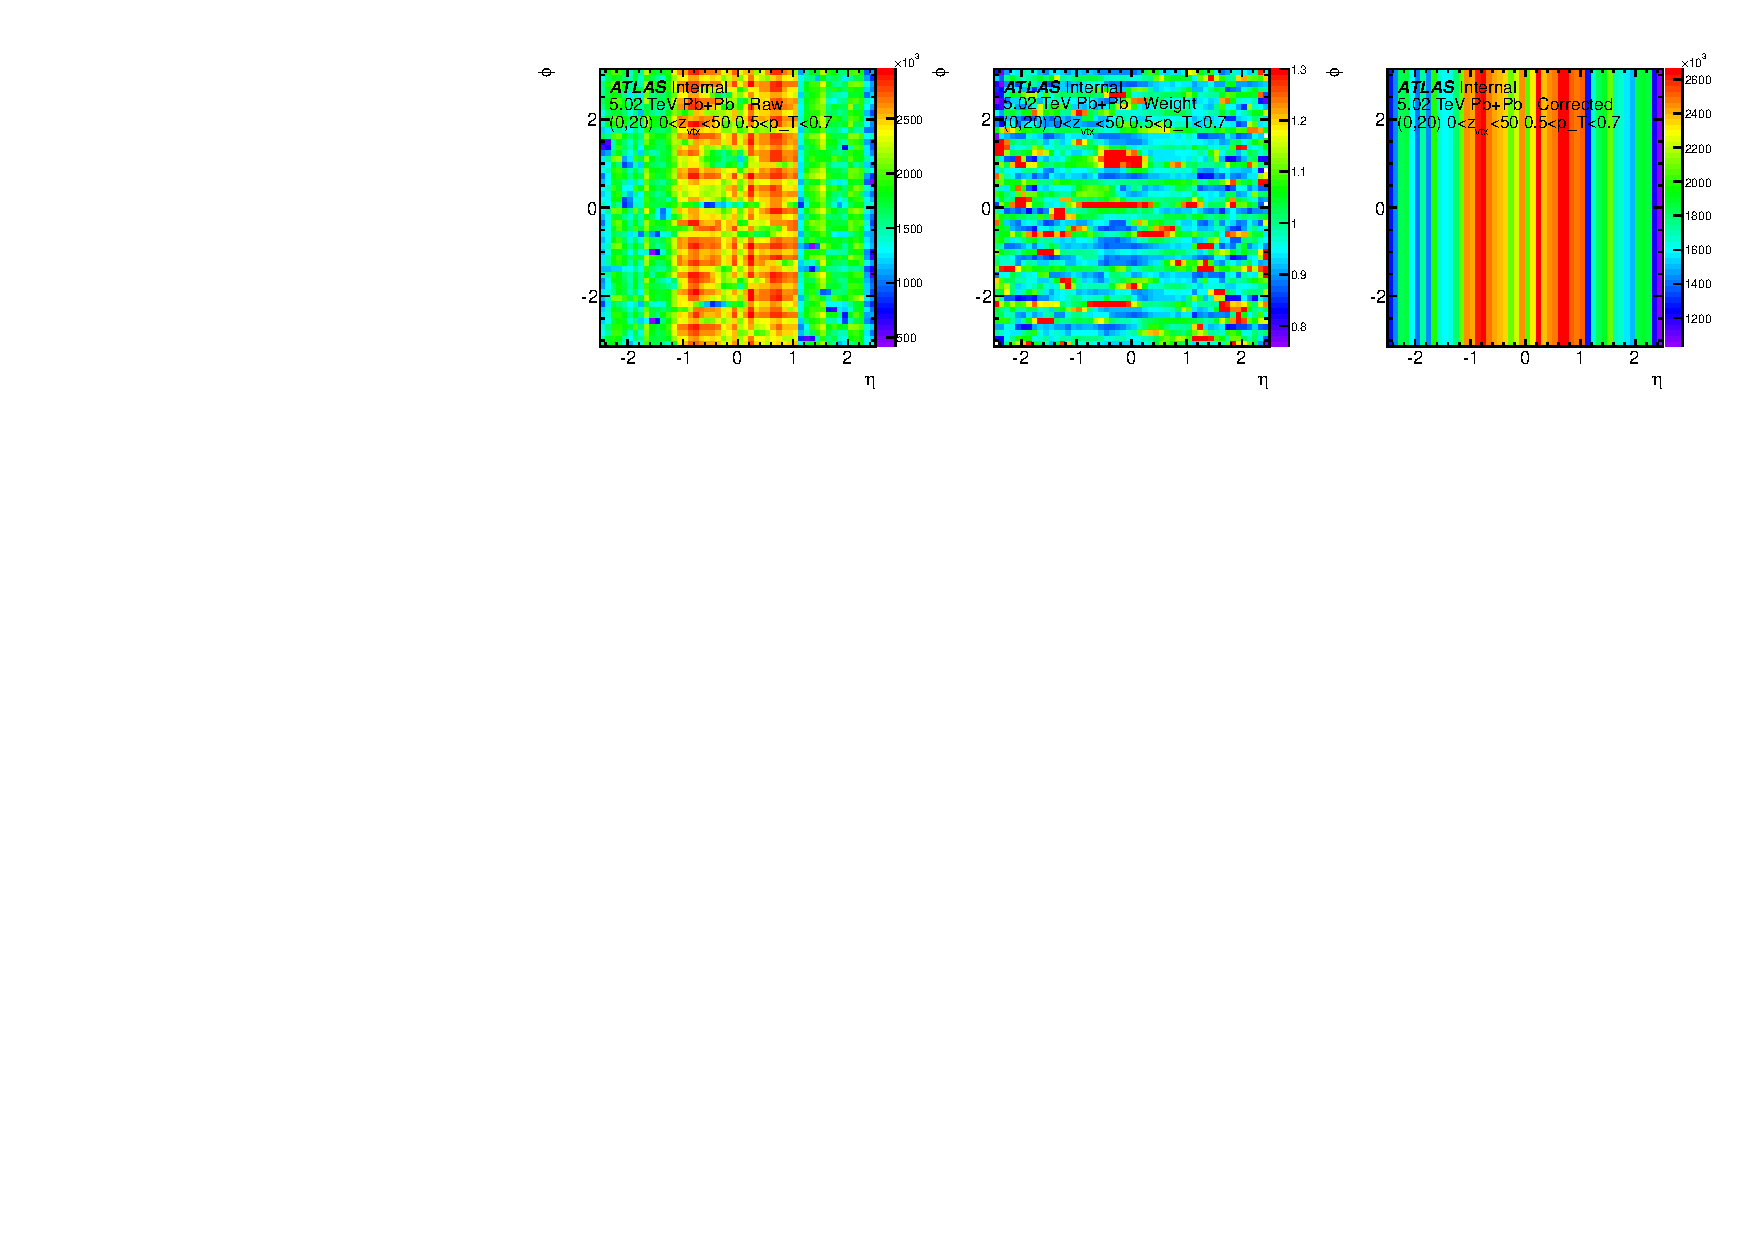
\includegraphics[width=.9\linewidth]{figs/sec_ana/cumuFlat_Cent0_Zvtx5_Chg1_Pt1.pdf}
\caption{Demonstration of flattening procedure with particles of different charges: top row is for negative-charged particles and bottom row is for positive-charged particles. Left column are the raw $(\eta,\phi)$ distributions, middle column are the estimated correction factor $w_{\phi}$, right column are the corrected $(\eta,\phi)$ distributions.}
\label{fig:cumuAna_FLAT_Chg}
\end{figure}

\begin{figure}[H]
\centering
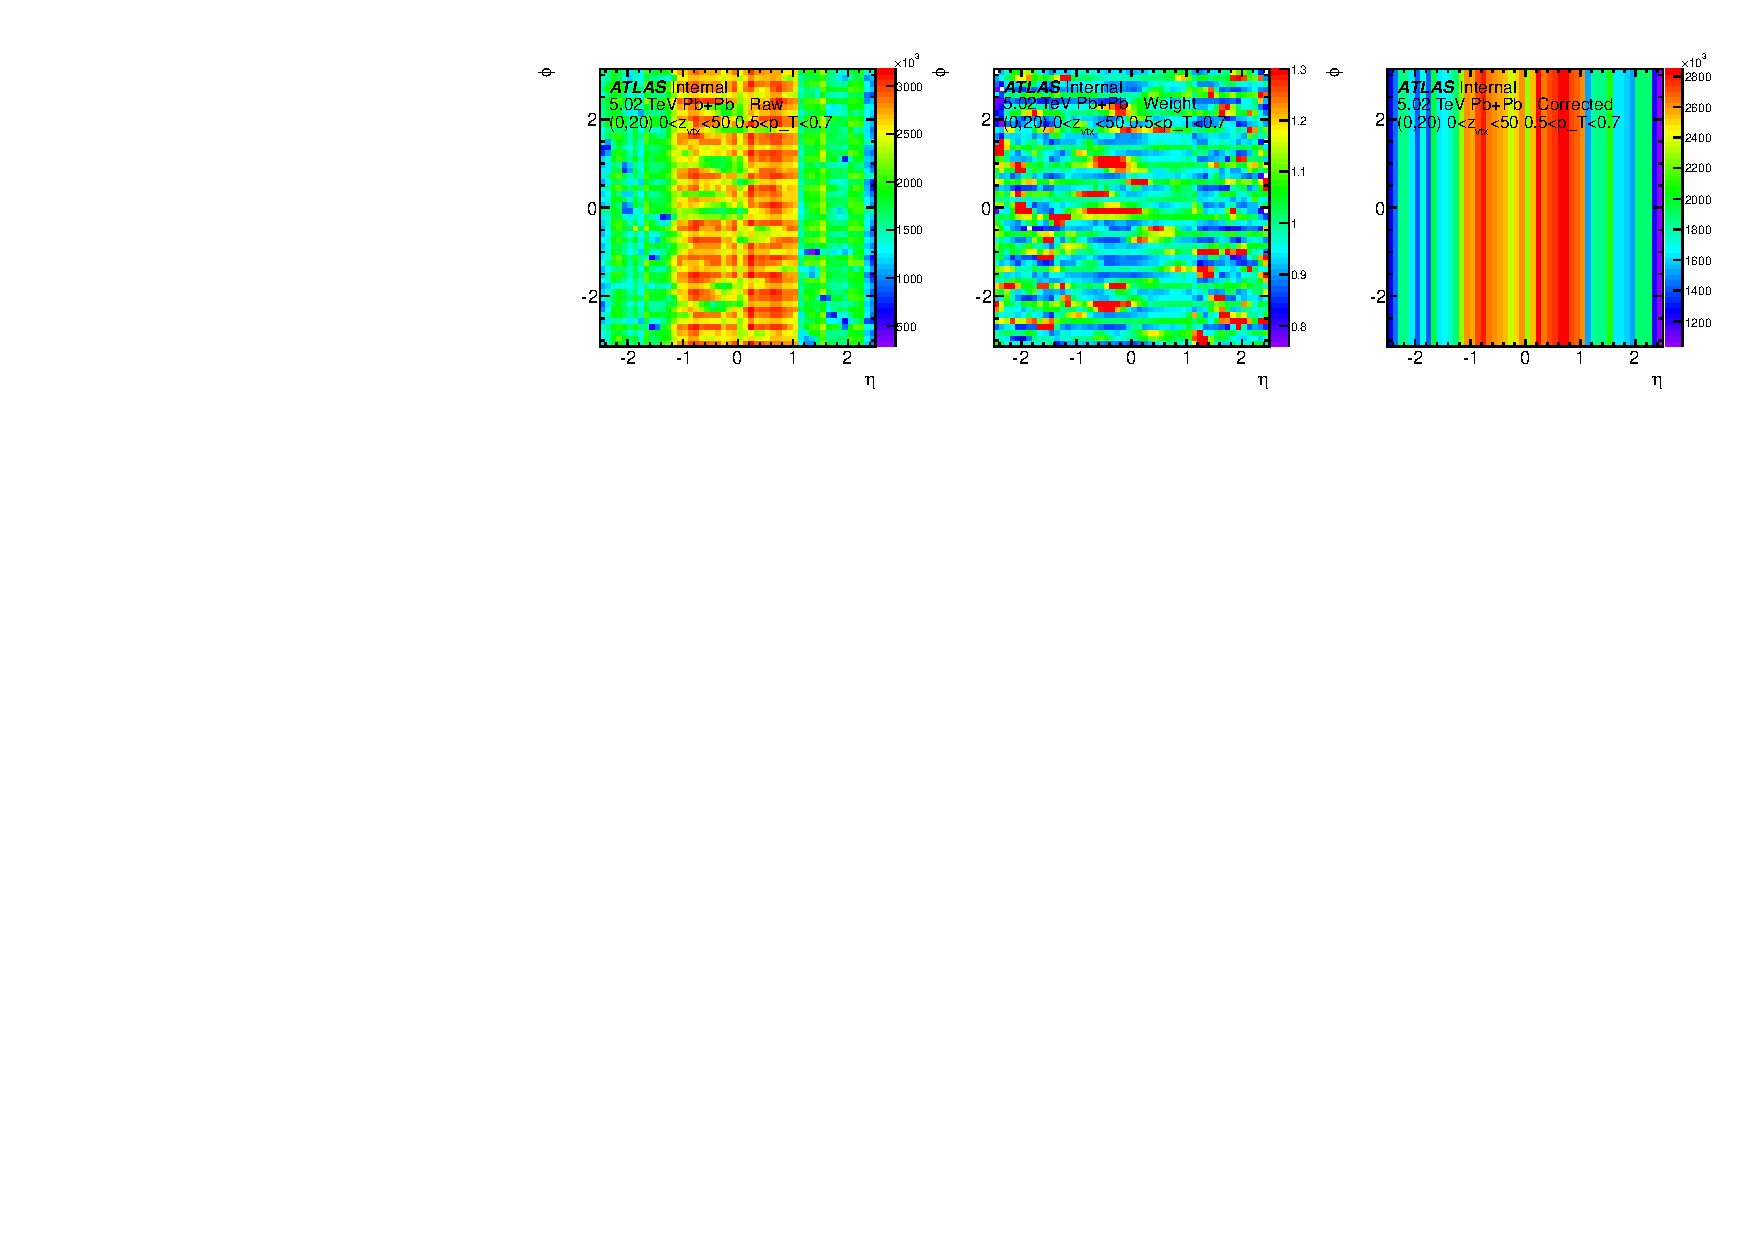
\includegraphics[width=.9\linewidth]{figs/sec_ana/cumuFlat_Cent0_Zvtx5_Chg0_Pt1.pdf}
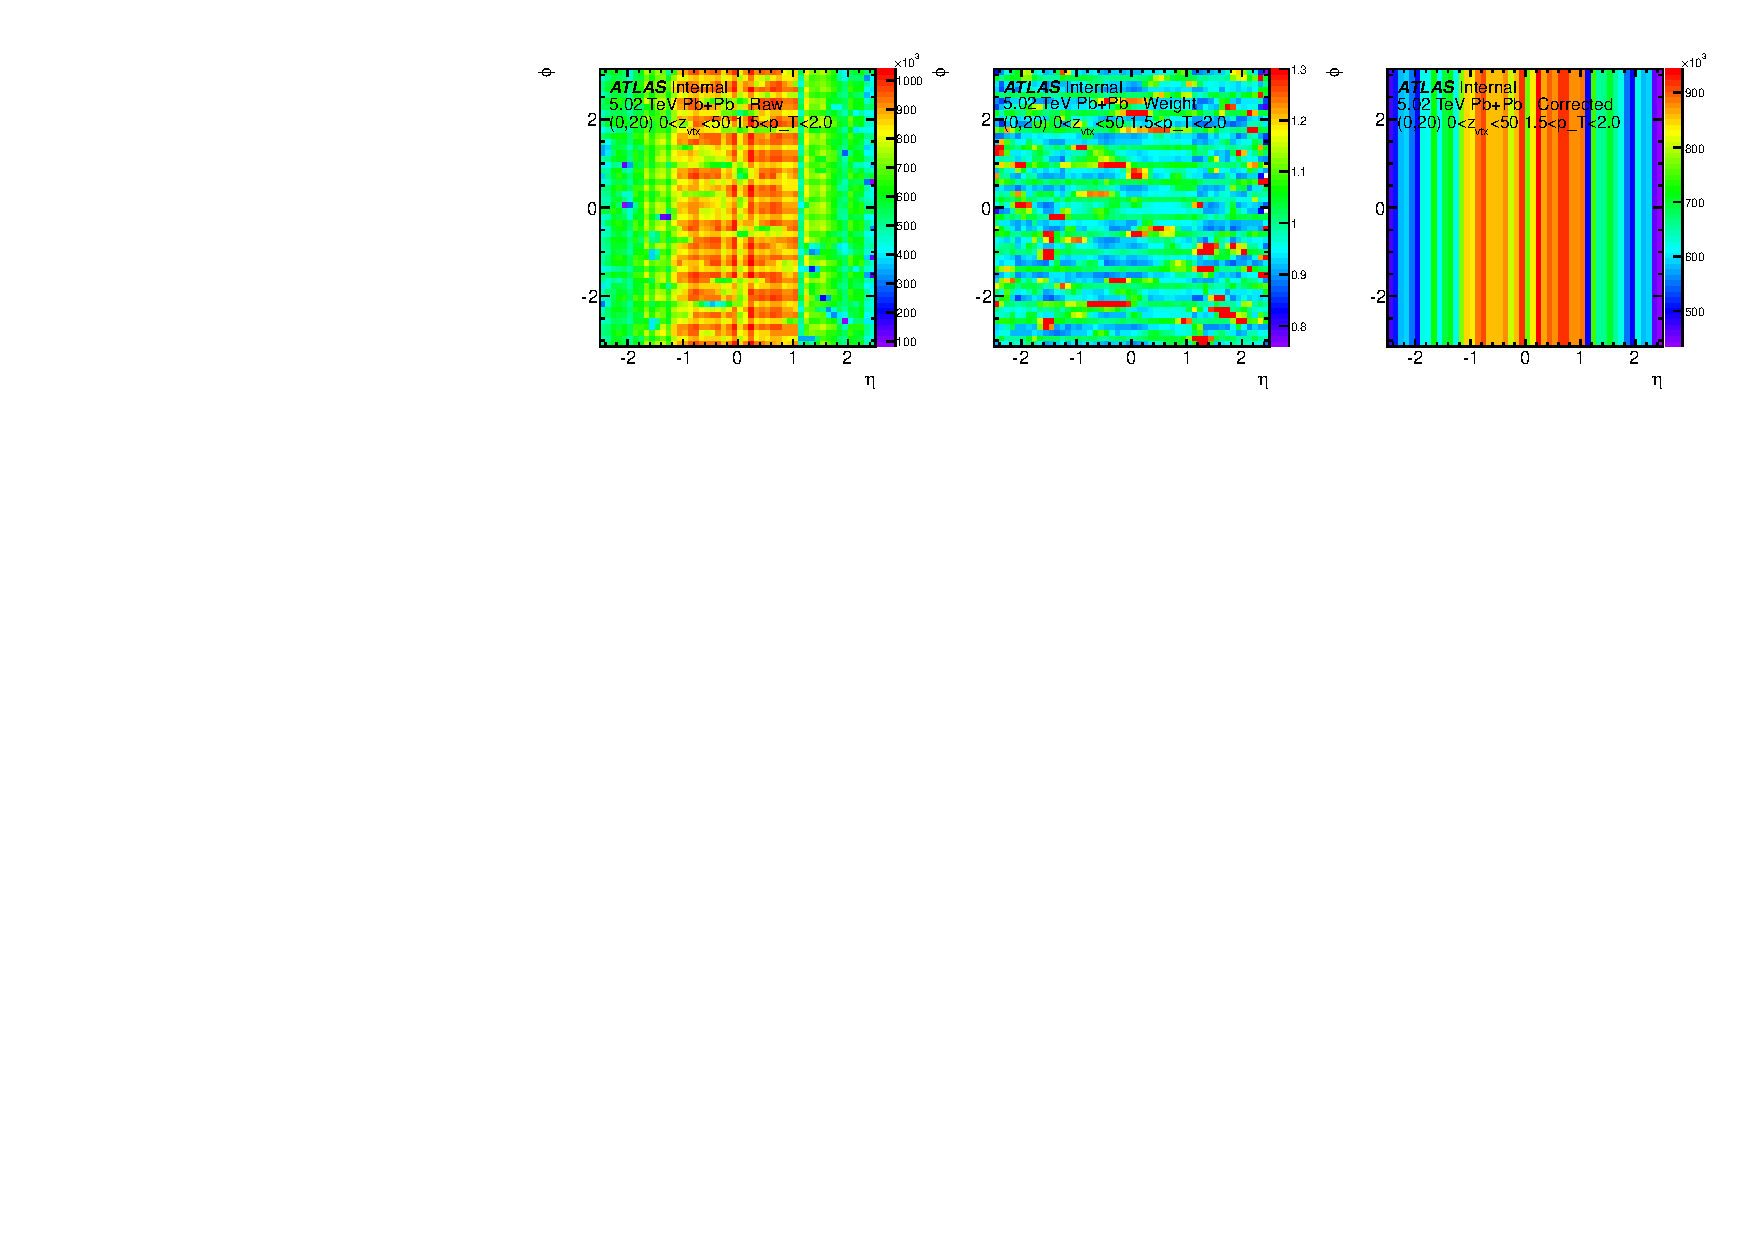
\includegraphics[width=.9\linewidth]{figs/sec_ana/cumuFlat_Cent0_Zvtx5_Chg0_Pt4.pdf}
\caption{Demonstration of flattening procedure with particles from different $p_\text{T}$ ranges: top row has $0.5<p_\text{T}<0.7$ GeV and bottom row has $1.5<p_\text{T}<2.0$ GeV. Left column are the raw $(\eta,\phi)$ distributions, middle column are the estimated correction factor $w_{\phi}$, right column are the corrected $(\eta,\phi)$ distributions. }
\label{fig:cumuAna_FLAT_Pt}
\end{figure}

In additional, the fluctuation of $z$ position of the primary vertex will cause the $N_{ch}$ distribution to shift in $\eta$. To compensate this effect, $w_\phi$ is also estimated in different $z_{vtx}$ ranges. Fig.~\ref{fig:cumuAna_FLAT_Zvtx} shows a comparison between -150 mm$<z_{vtx}<$-100 mm and 100 mm$<z_{vtx}<$150 mm. From the left column, it is clear that the $\eta$ distributions are shifted together with $z_{vtx}$ position, which means that a $z_{vtx}$-dependent $w_\phi$ correction is needed.

Furthermore, the $w_\phi$ corrections are also evaluated for negative- and positive-charged particles separately, as shown in Fig.~\ref{fig:cumuAna_FLAT_Chg}. From the raw distribution, differences have already been observed: there are slightly more holes for positive particles than negative ones.

In the end, Fig.~\ref{fig:cumuAna_FLAT_Pt} shows the comparison of $w_\phi$ estimated from particles in two different $p_\text{T}$ ranges: $0.3<p_\text{T}<0.5$ GeV and $1.5<p_\text{T}<2.0$ GeV. As a results, particles with higher $p_\text{T}$ are more uniformly distributed, which is consistent with the fact that tracking efficiency increases towards higher $p_\text{T}$.



\subsection{Event class}
Event-by-event multi-particle correlation $corr_{n}\{2k\}$ is averaged within bunch of similar events, which are denoted as event class. Since cumulant measures the flow fluctuation in certain event class, how event class is defined will have an effect on the cumulant magnitude. In previous ATLAS paper on cumulant in small systems, we have shown that even the sign of cumulant can change if the event class definition is changed. In this section, we will discuss the definition of event class in this analysis and its potential impact on the cumulant results.

Since flow in the final stage is strongly correlated with the eccentricity from the initial stage, an optimal quantity to model the eccentricity changing would be centrality, which reflects the overlapping region of the two nucleus. In heavy ion collision, since centrality is not a direct-measurable quantity, total transverse energy $E_\text{T}$ in the FCal detector is used as an indicator for centrality, which means the centrality percentile is calculated based on the FCal $E_\text{T}$ distribution (see the Dataset section for details). In this analysis, the default event class will be defined by centrality.

The following question is how large the event class bin width should be. In principle, narrower bin width is always preferred, since wider bin width will include events from different centralities, which can result in different flow fluctuation. However, there will be not enough events to calculate the higher order cumulants if the bin width is too narrow. In practice we choose $1\%$ centrality percentile as the default event class bin width.

To show that $1\%$ bin width will not introduce any bias to the measurement, we have also tested the following bin widths:
\begin{itemize}
\item Event class bin width: $2\%$;
\item Event class bin width: $5\%$;
\item Event class bin width: $10\%$;
\end{itemize}
and the results will be discussed in the systematic section.

As discussed in the methodology section, even though the event class bin width is only $1\%$ centrality, neighbouring bins will be merged together at the cumulant level to increase the statistics. Note that since the re-bin is performed on the cumulant, it does not change the underlying flow fluctuation.

The event class definition is specially treated in the ultra-central collision, simply because $1\%$ centrality bin width is not narrow enough to constrain the fluctuation of flow. Instead, the following event class criteria are used:
\begin{itemize}
\item Event class defined by FCal $E_\text{T}$, with bin width $=6$ GeV;
\item Event class defined by number of reconstructed tracks $N_{ch}^{rec}$, with $p_\text{T}$ range always $0.5<p_\text{T}<5.0$ GeV, no matter the $p_\text{T}$ range for the cumulant calculation. The bin width is 5 track;
\end{itemize}
where the purpose of the second criteria is to evaluate the flow fluctuation by changing the centrality definition, which will be discussed in the results section.

\begin{figure}[H]
\centering
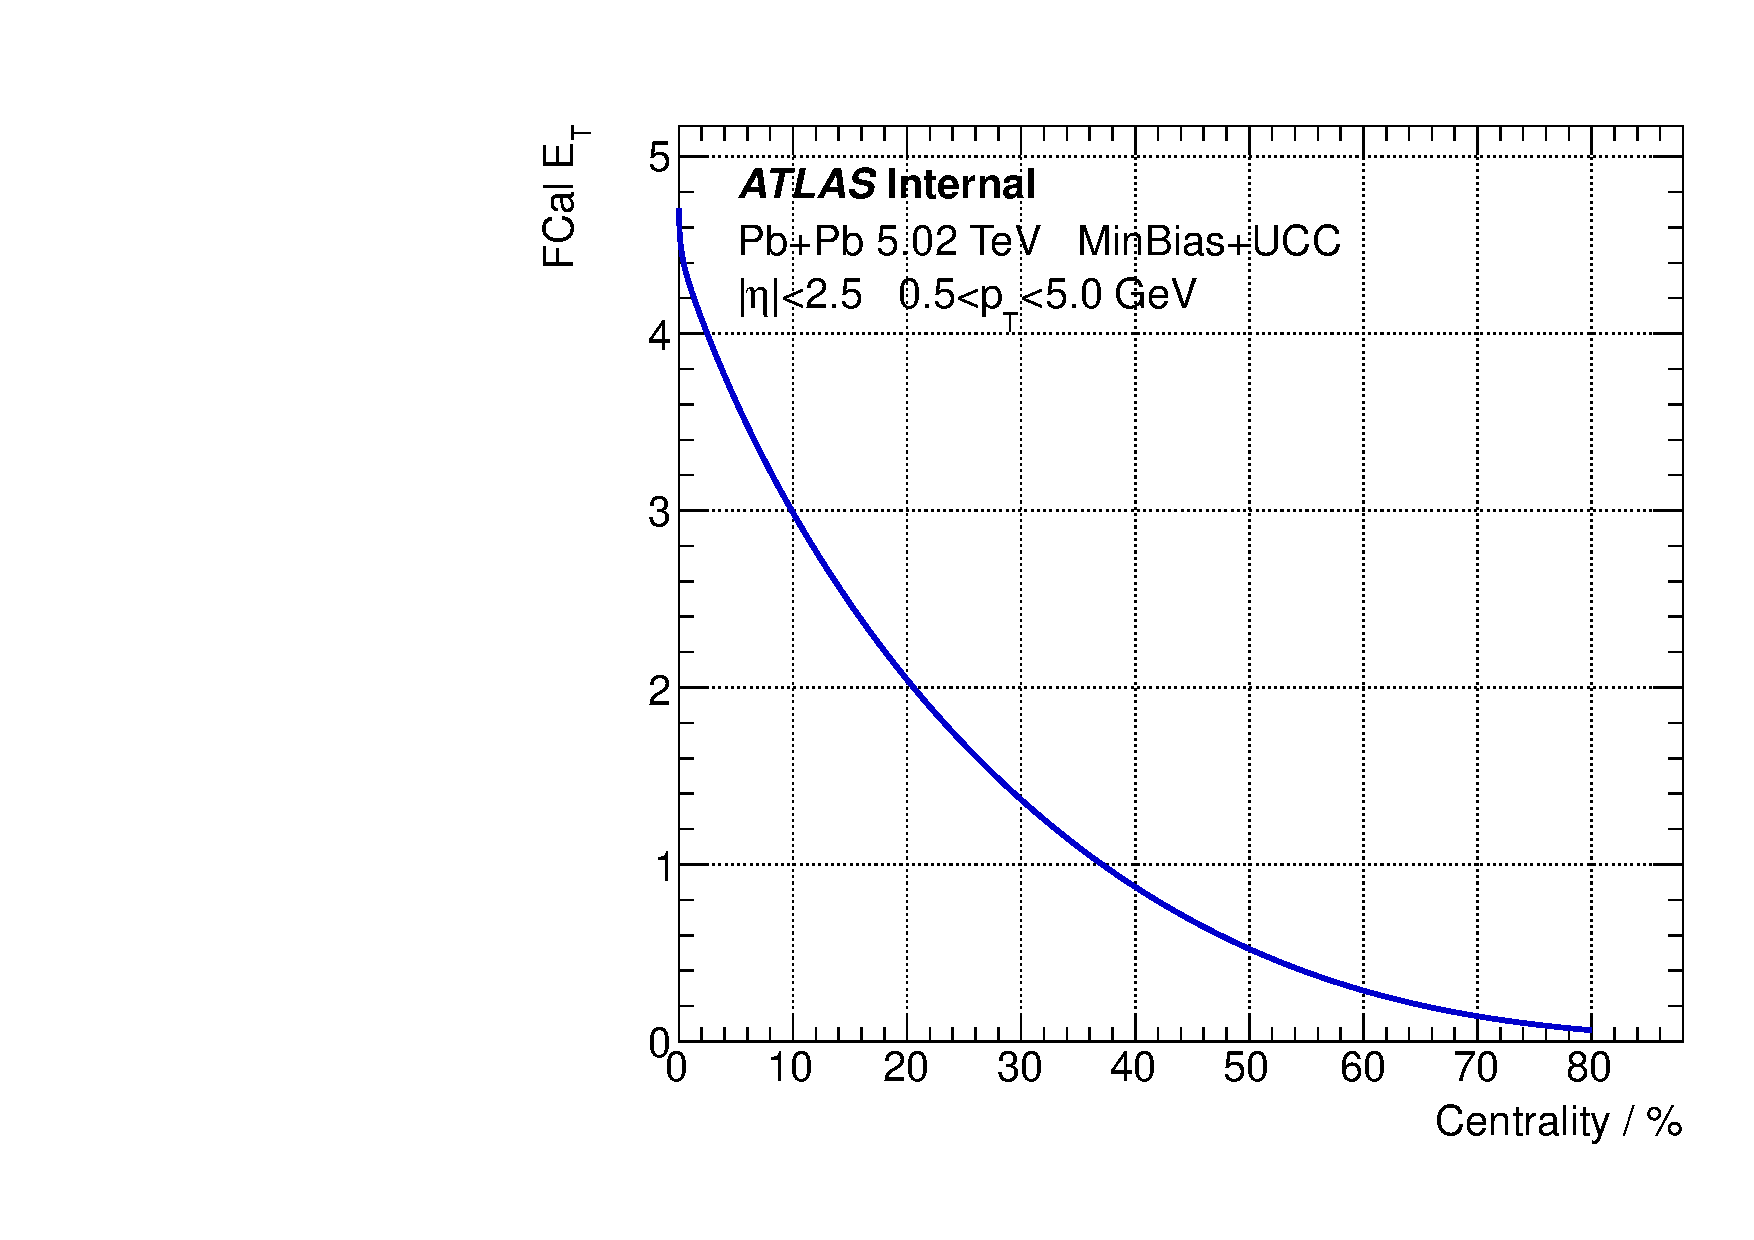
\includegraphics[width=.32\linewidth]{figs/sec_ana/cvtMap_cent_fcal.pdf}
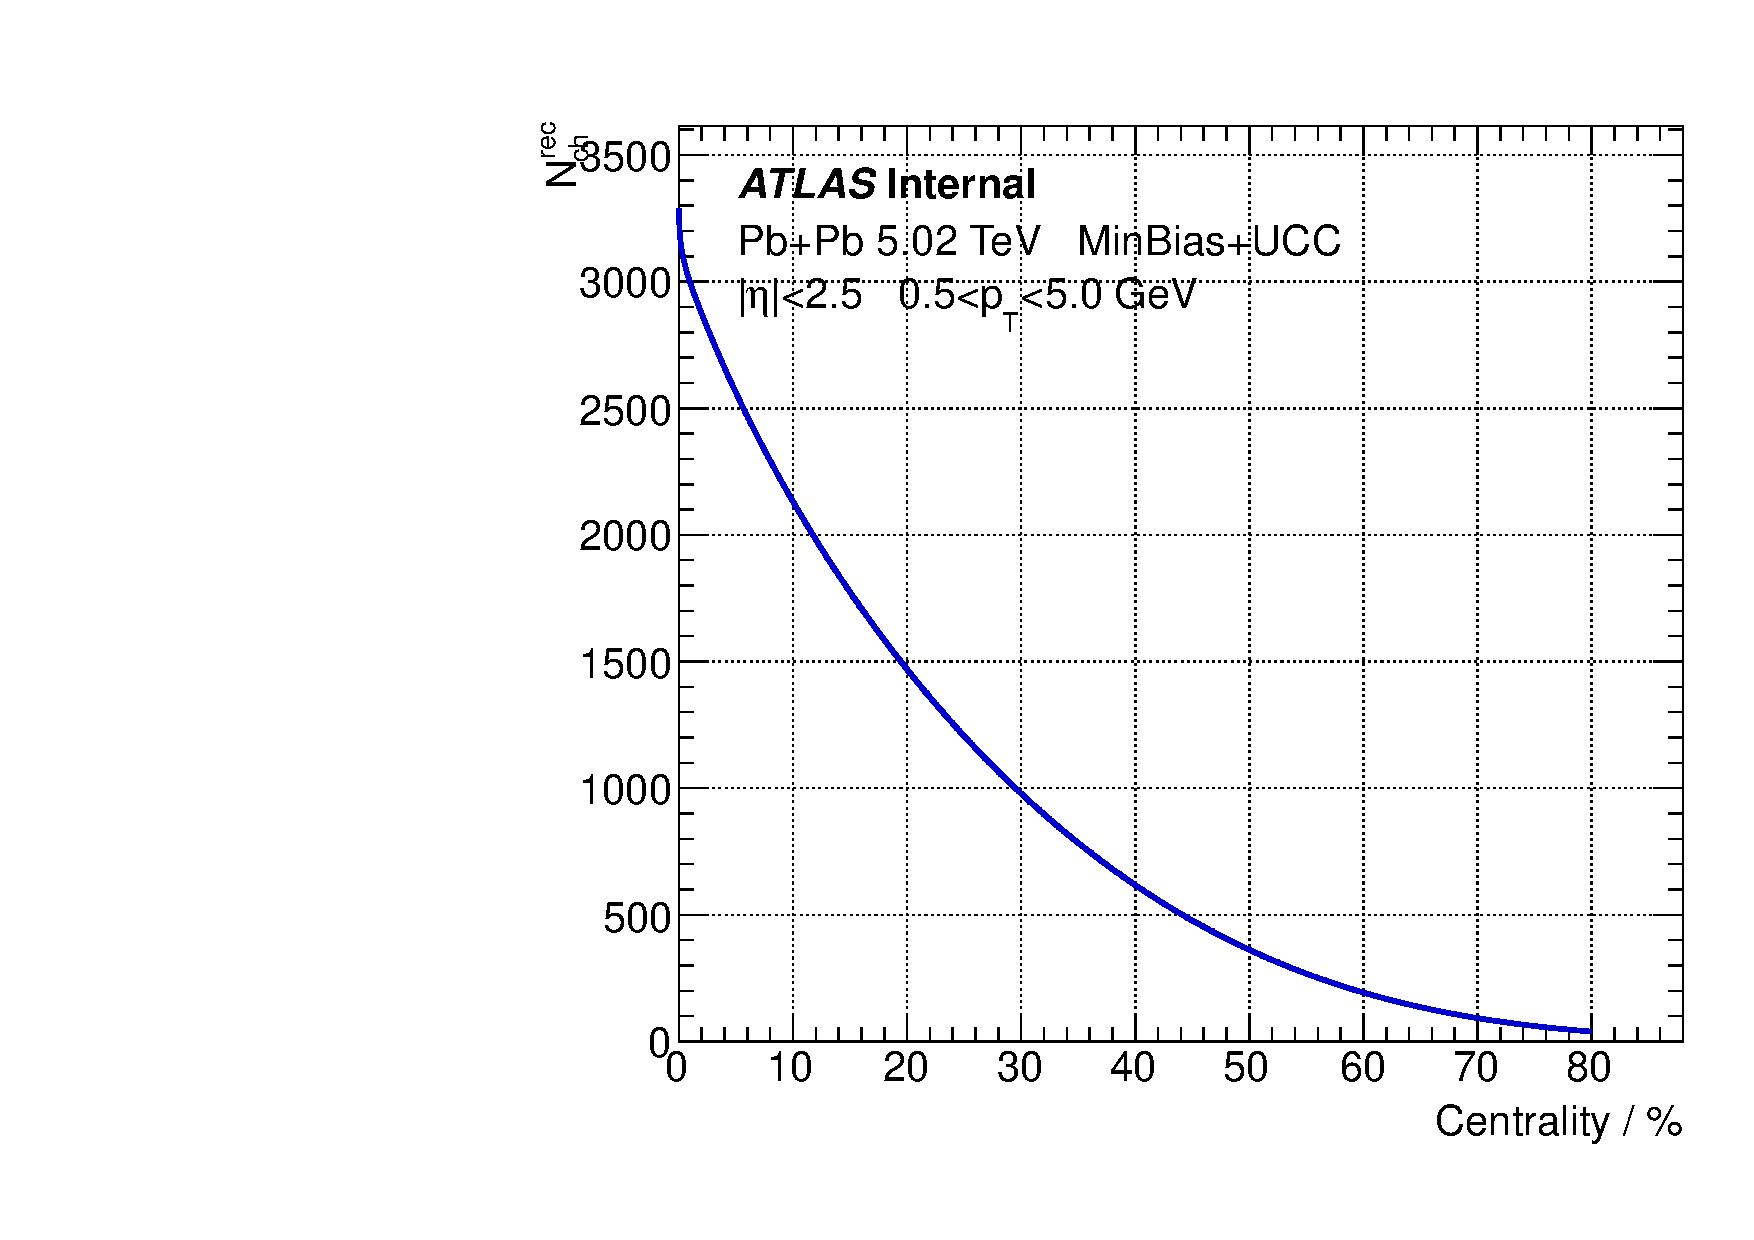
\includegraphics[width=.32\linewidth]{figs/sec_ana/cvtMap_cent_NchRec.pdf}
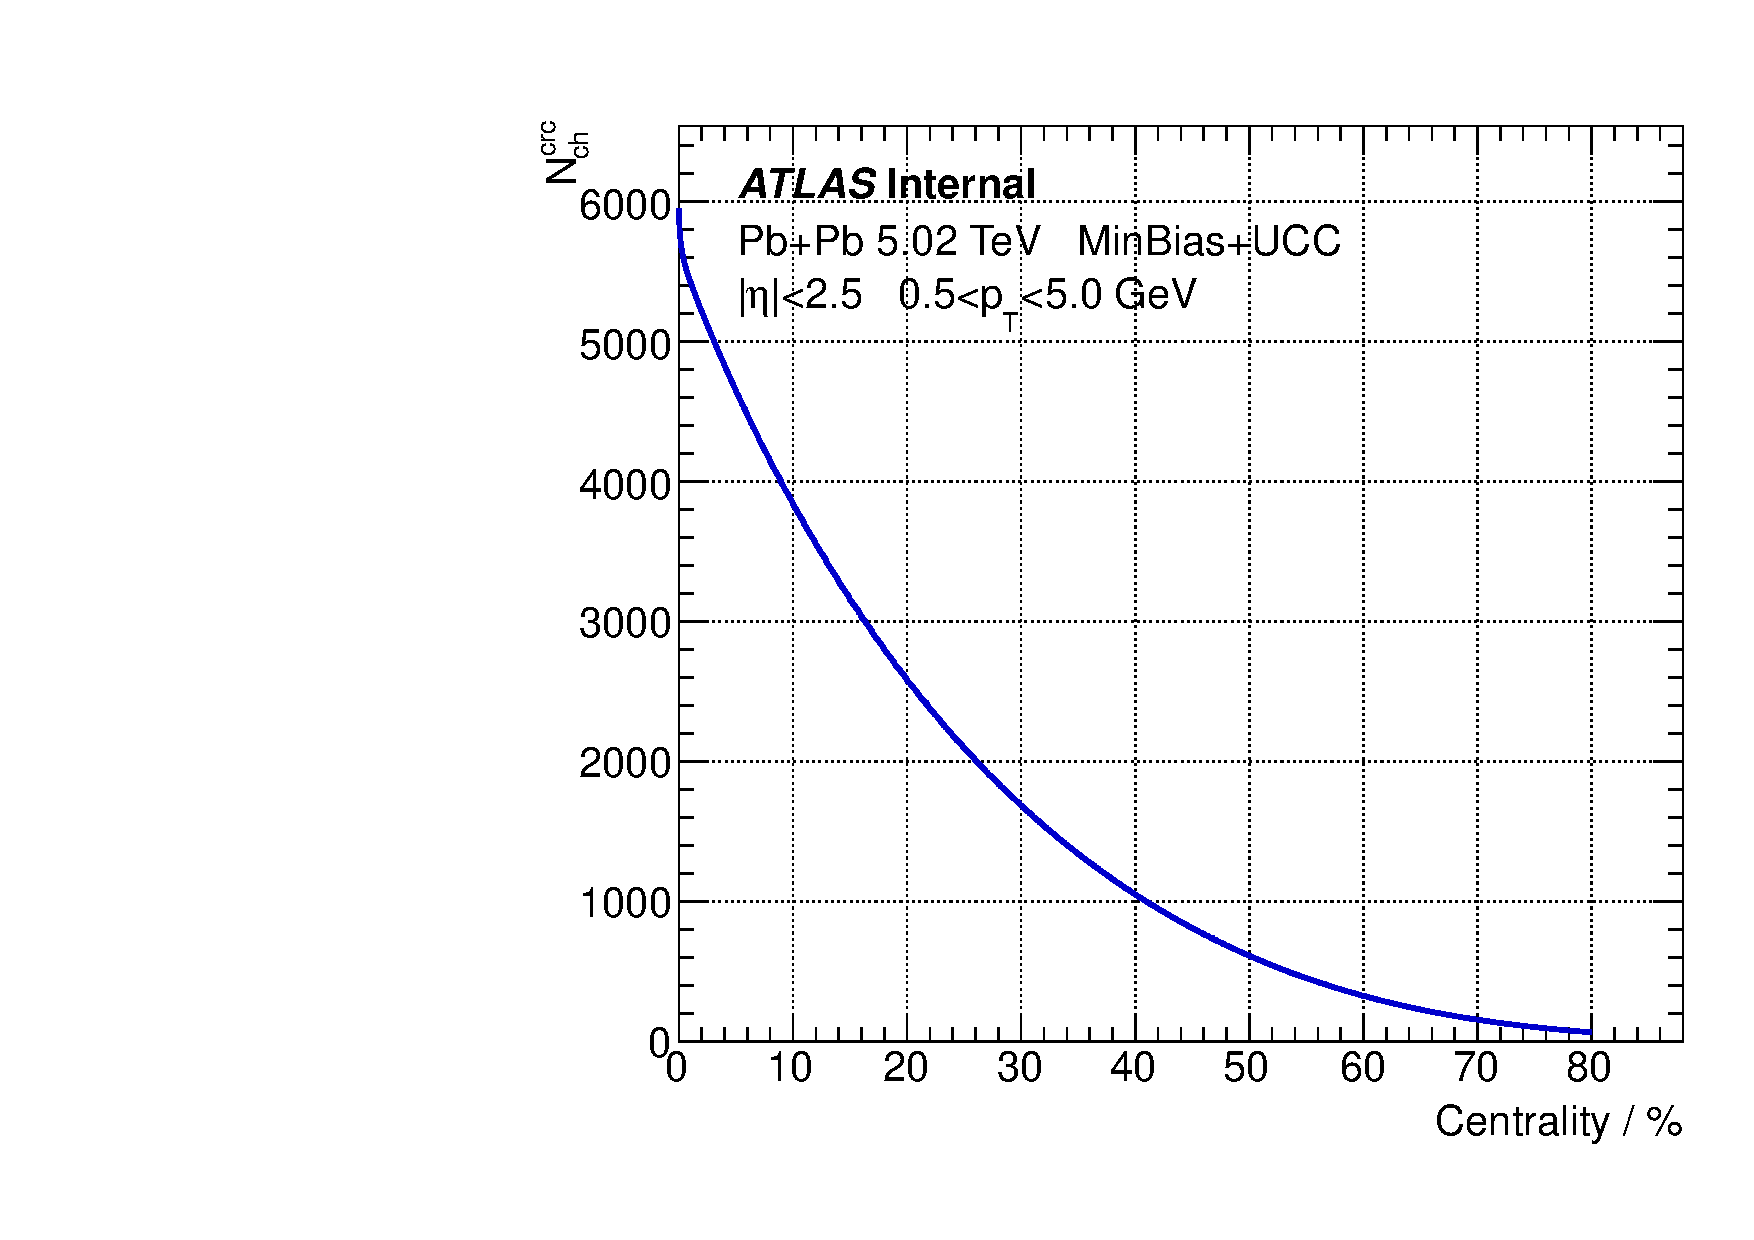
\includegraphics[width=.32\linewidth]{figs/sec_ana/cvtMap_cent_NchCrc.pdf}
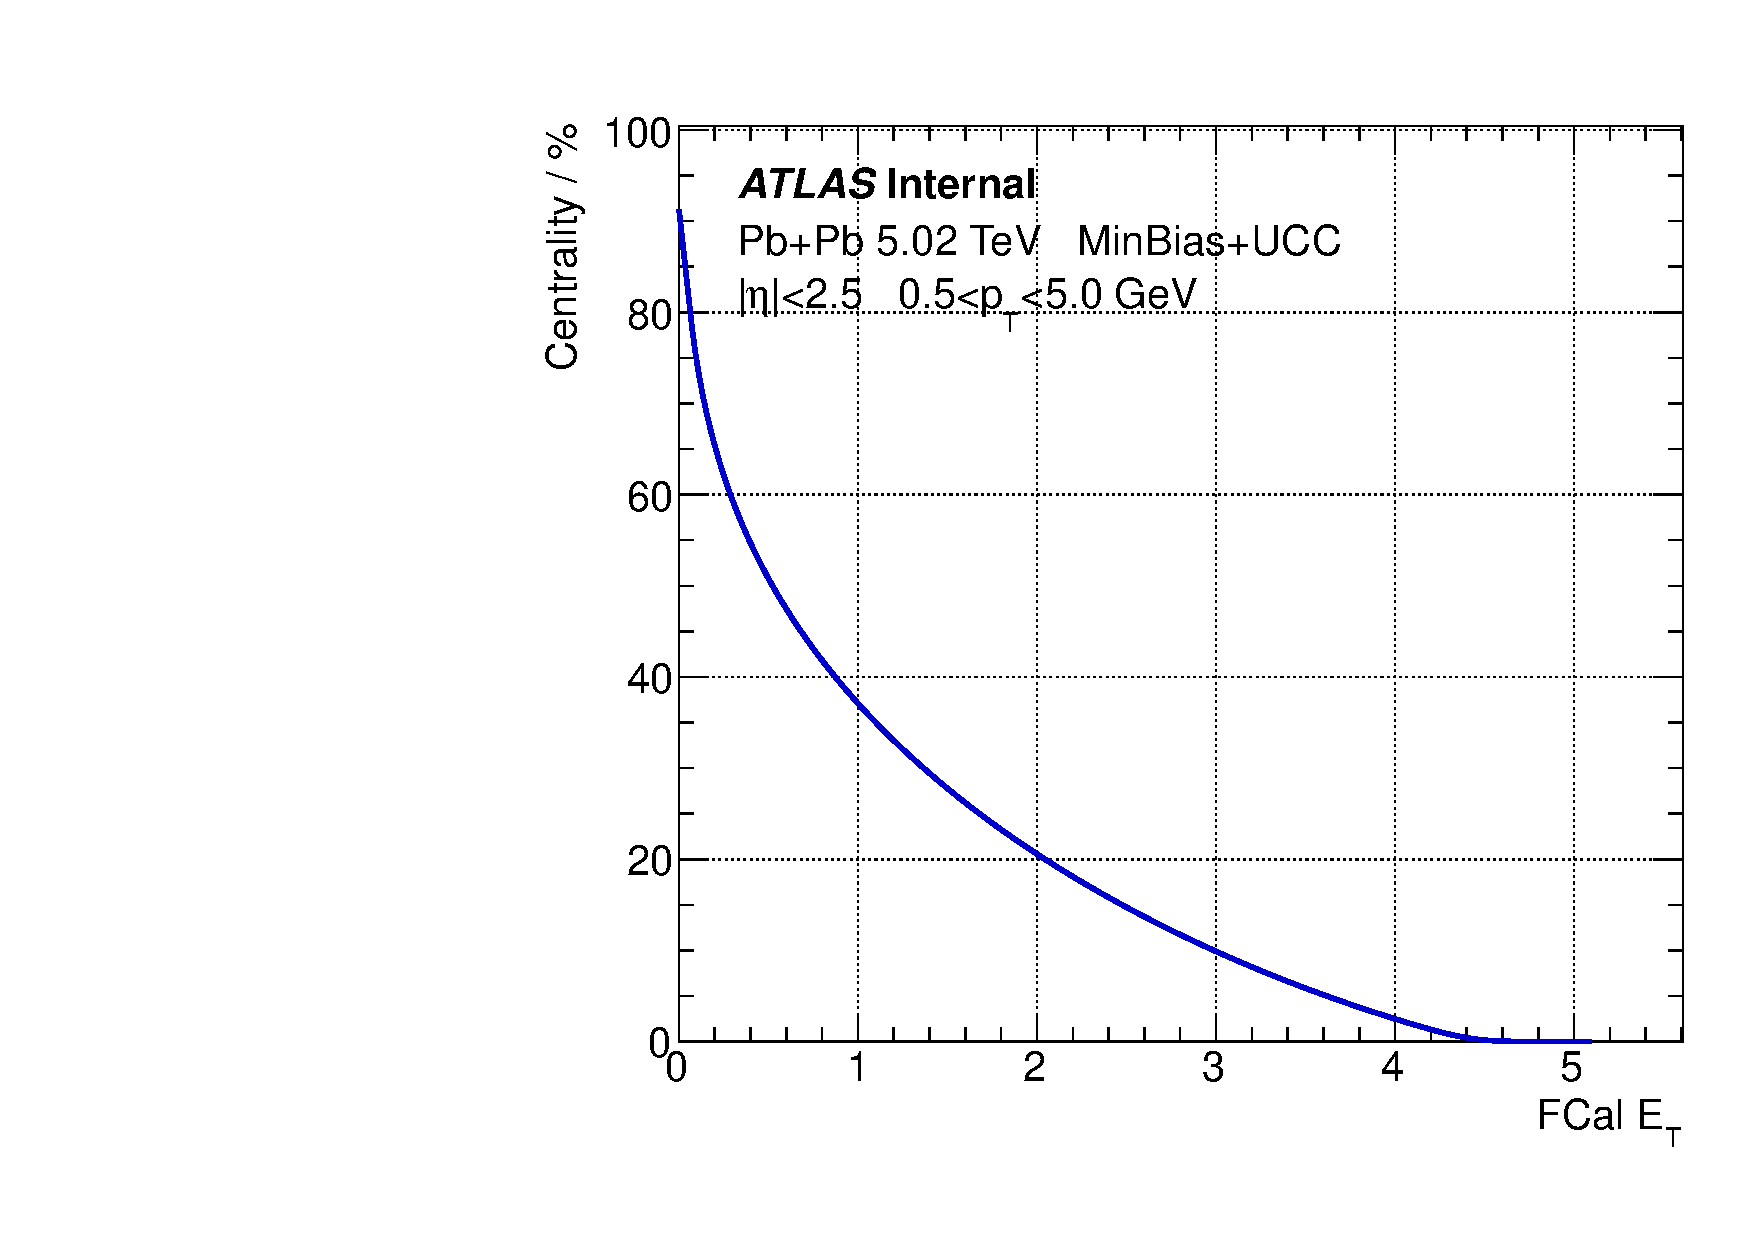
\includegraphics[width=.32\linewidth]{figs/sec_ana/cvtMap_fcal_cent.pdf}
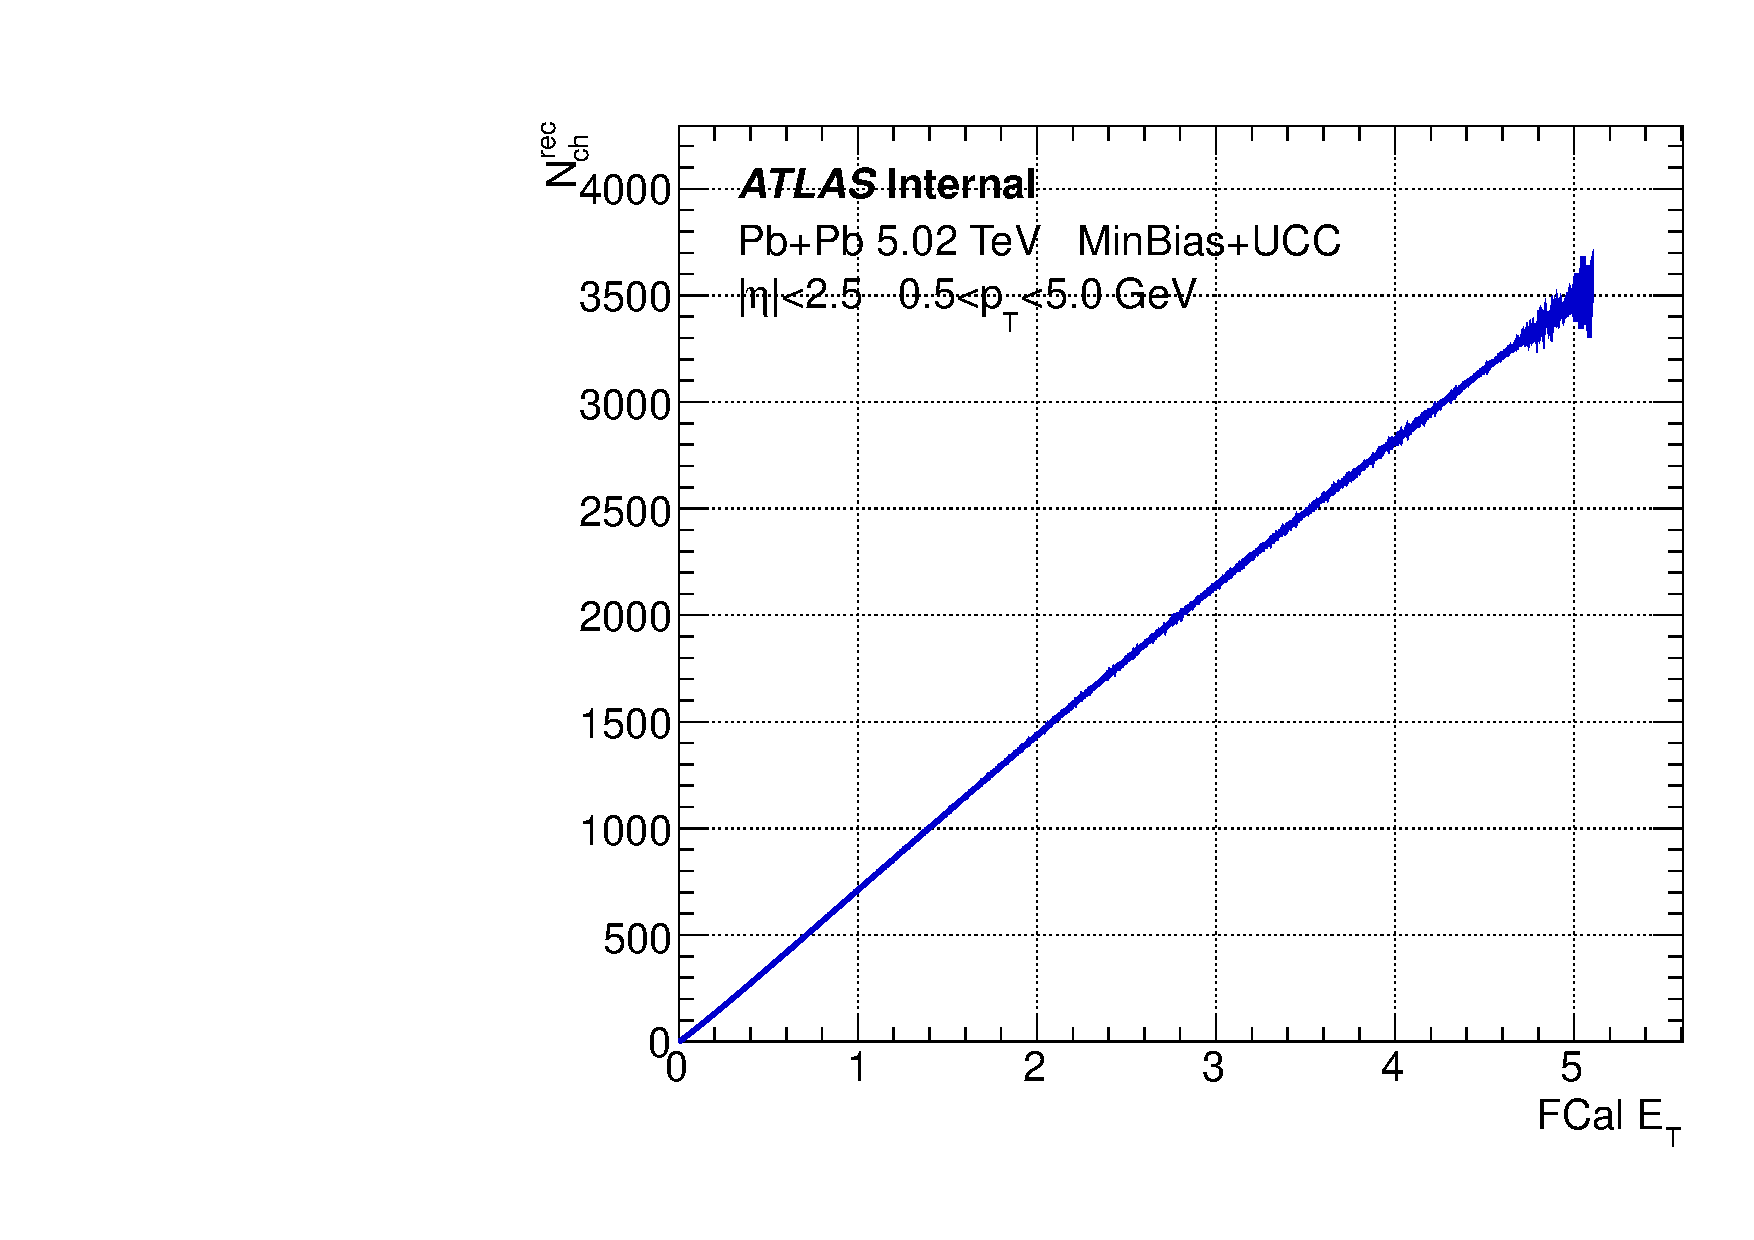
\includegraphics[width=.32\linewidth]{figs/sec_ana/cvtMap_fcal_NchRec.pdf}
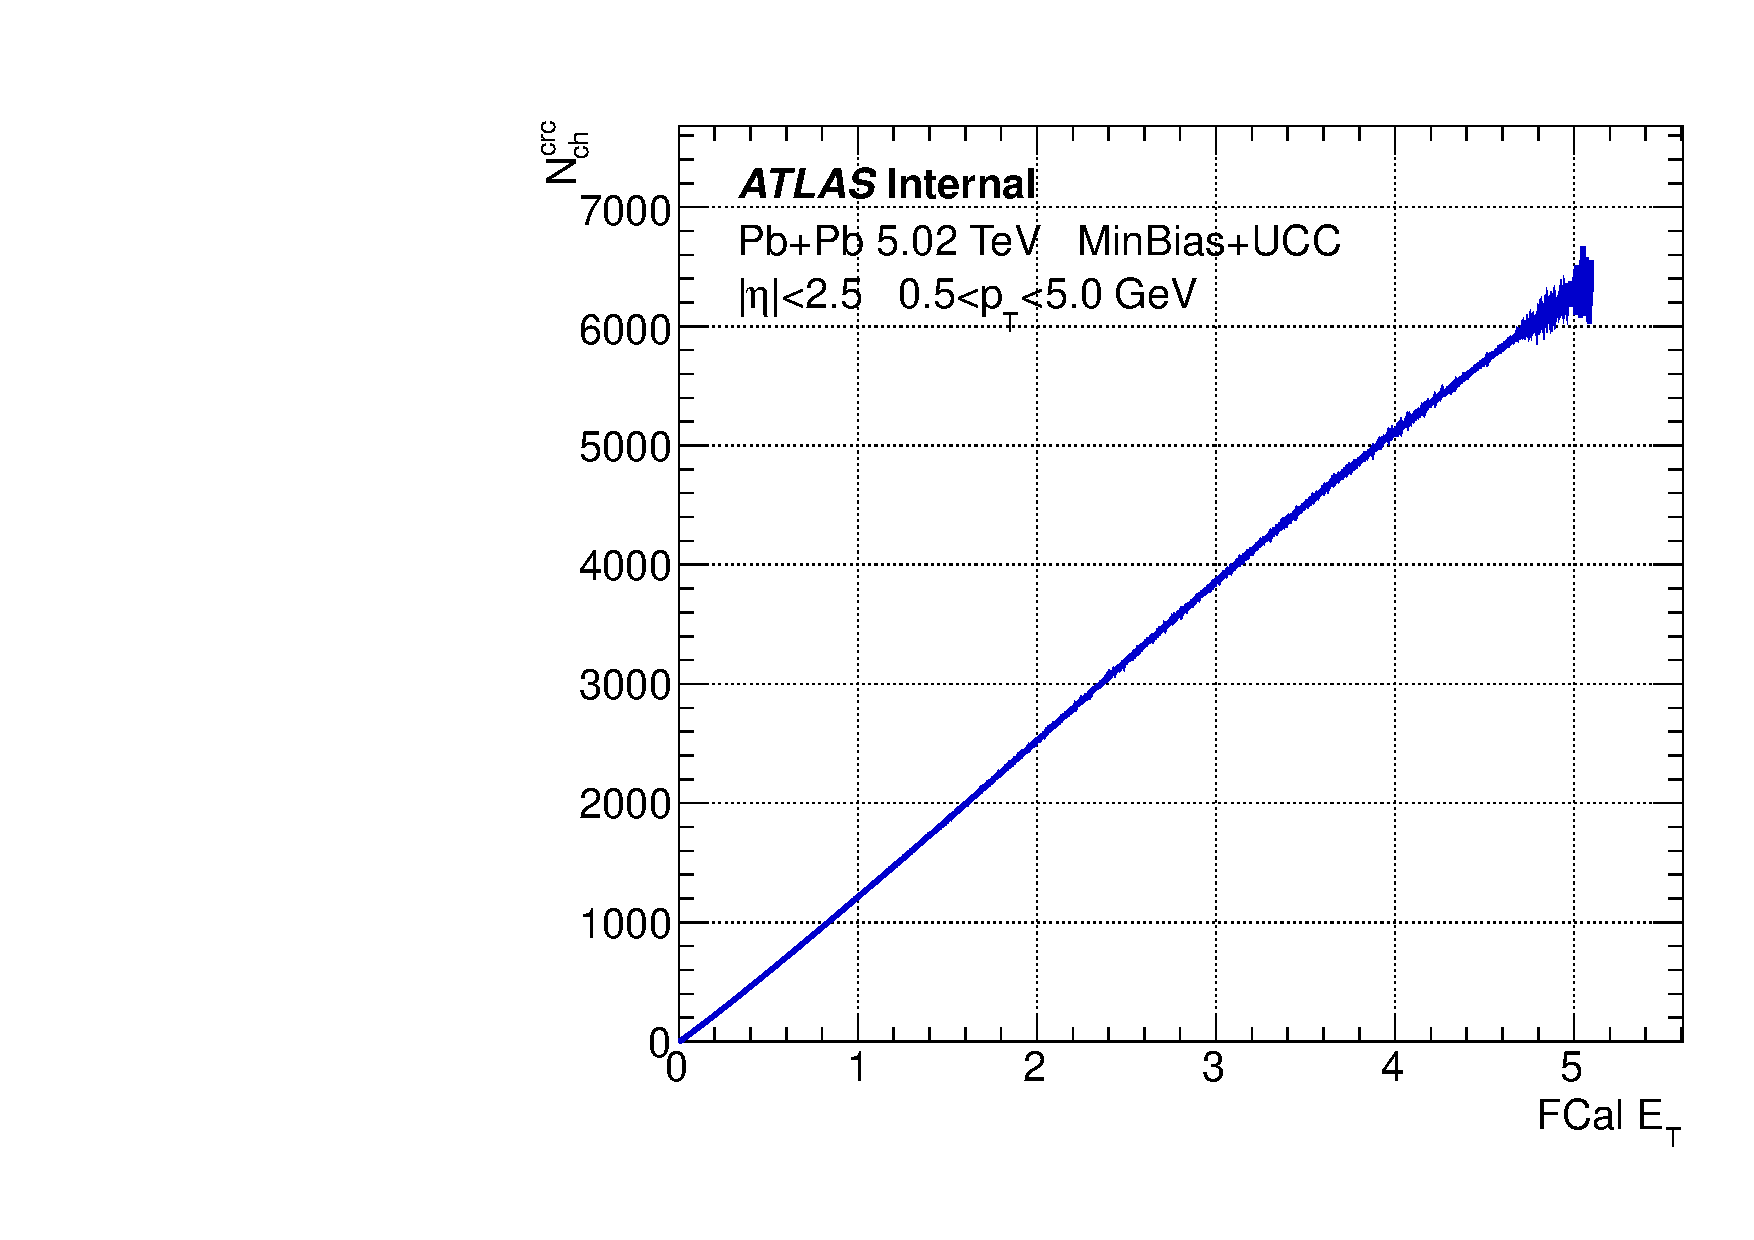
\includegraphics[width=.32\linewidth]{figs/sec_ana/cvtMap_fcal_NchCrc.pdf}
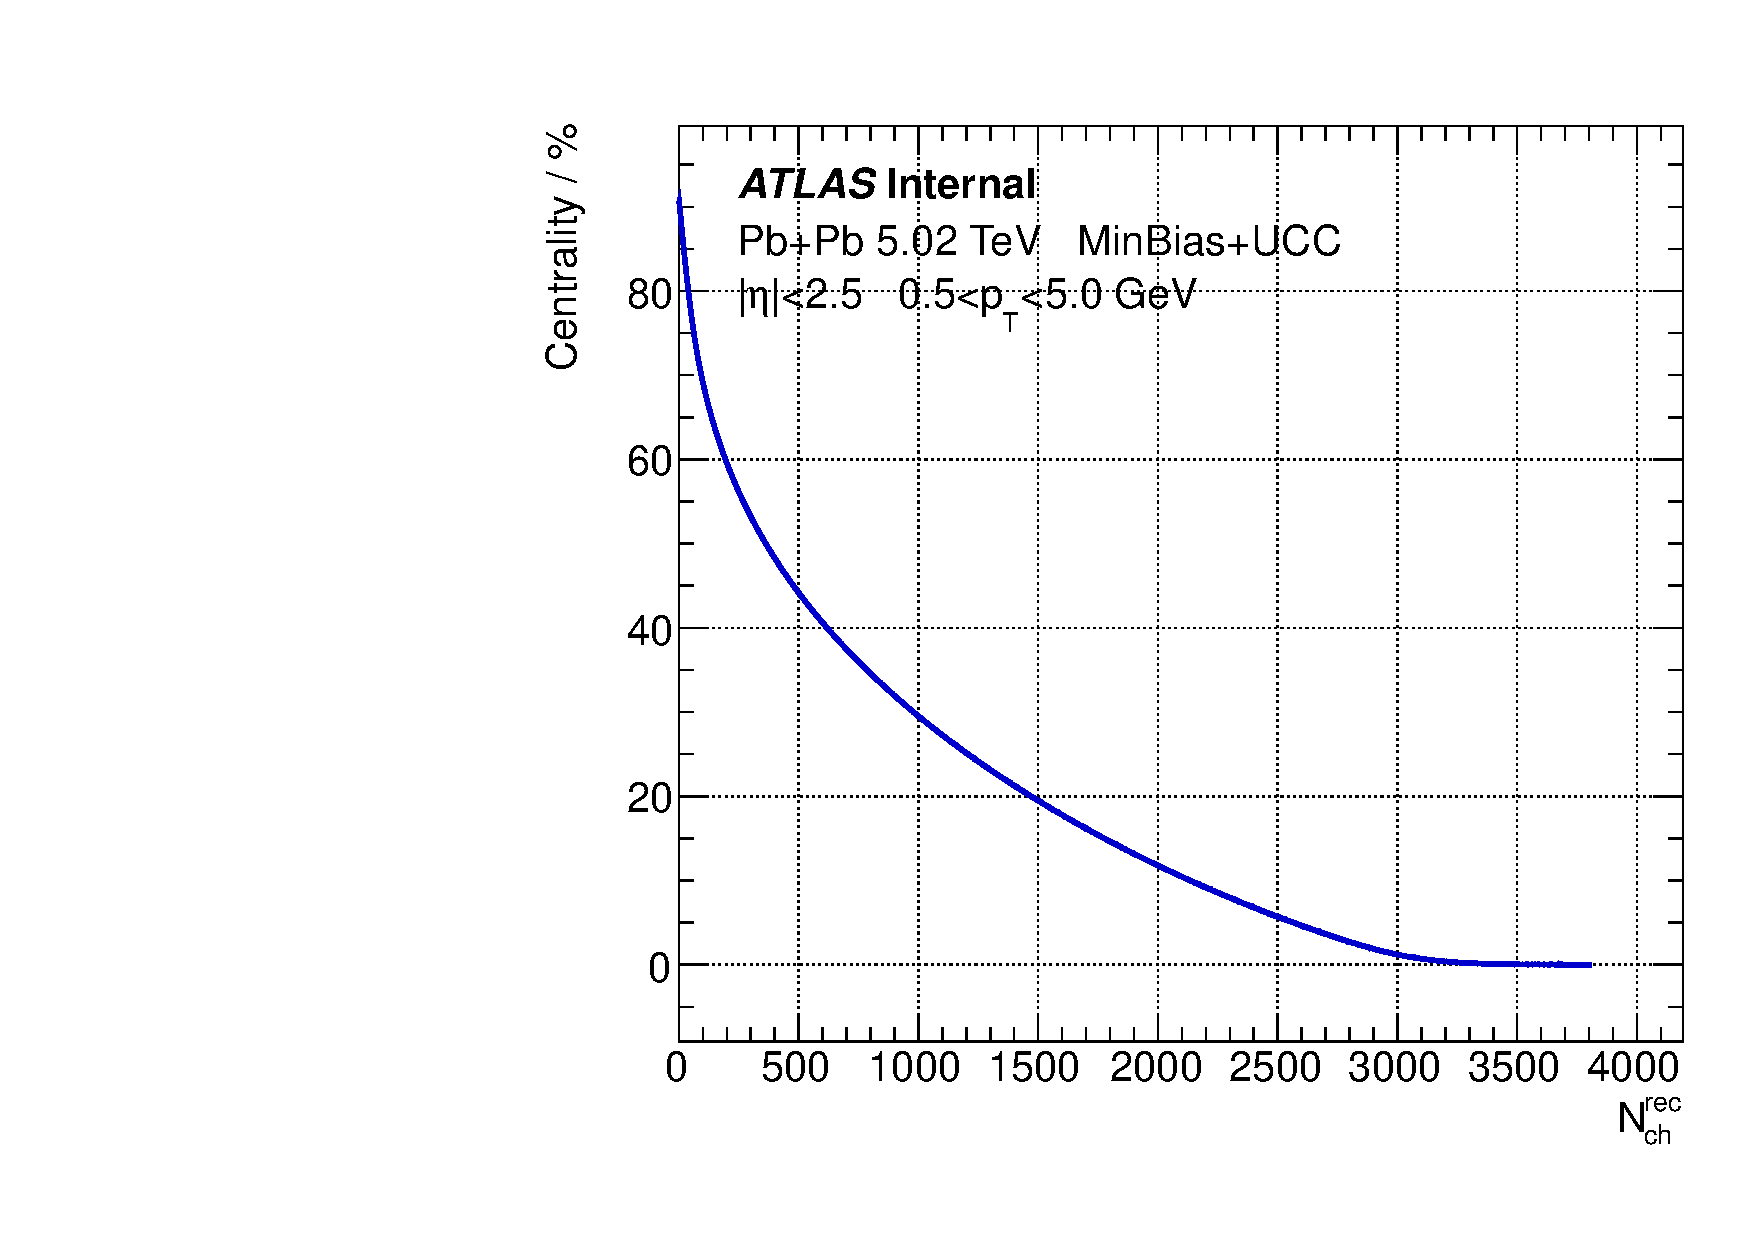
\includegraphics[width=.32\linewidth]{figs/sec_ana/cvtMap_NchRec_cent.pdf}
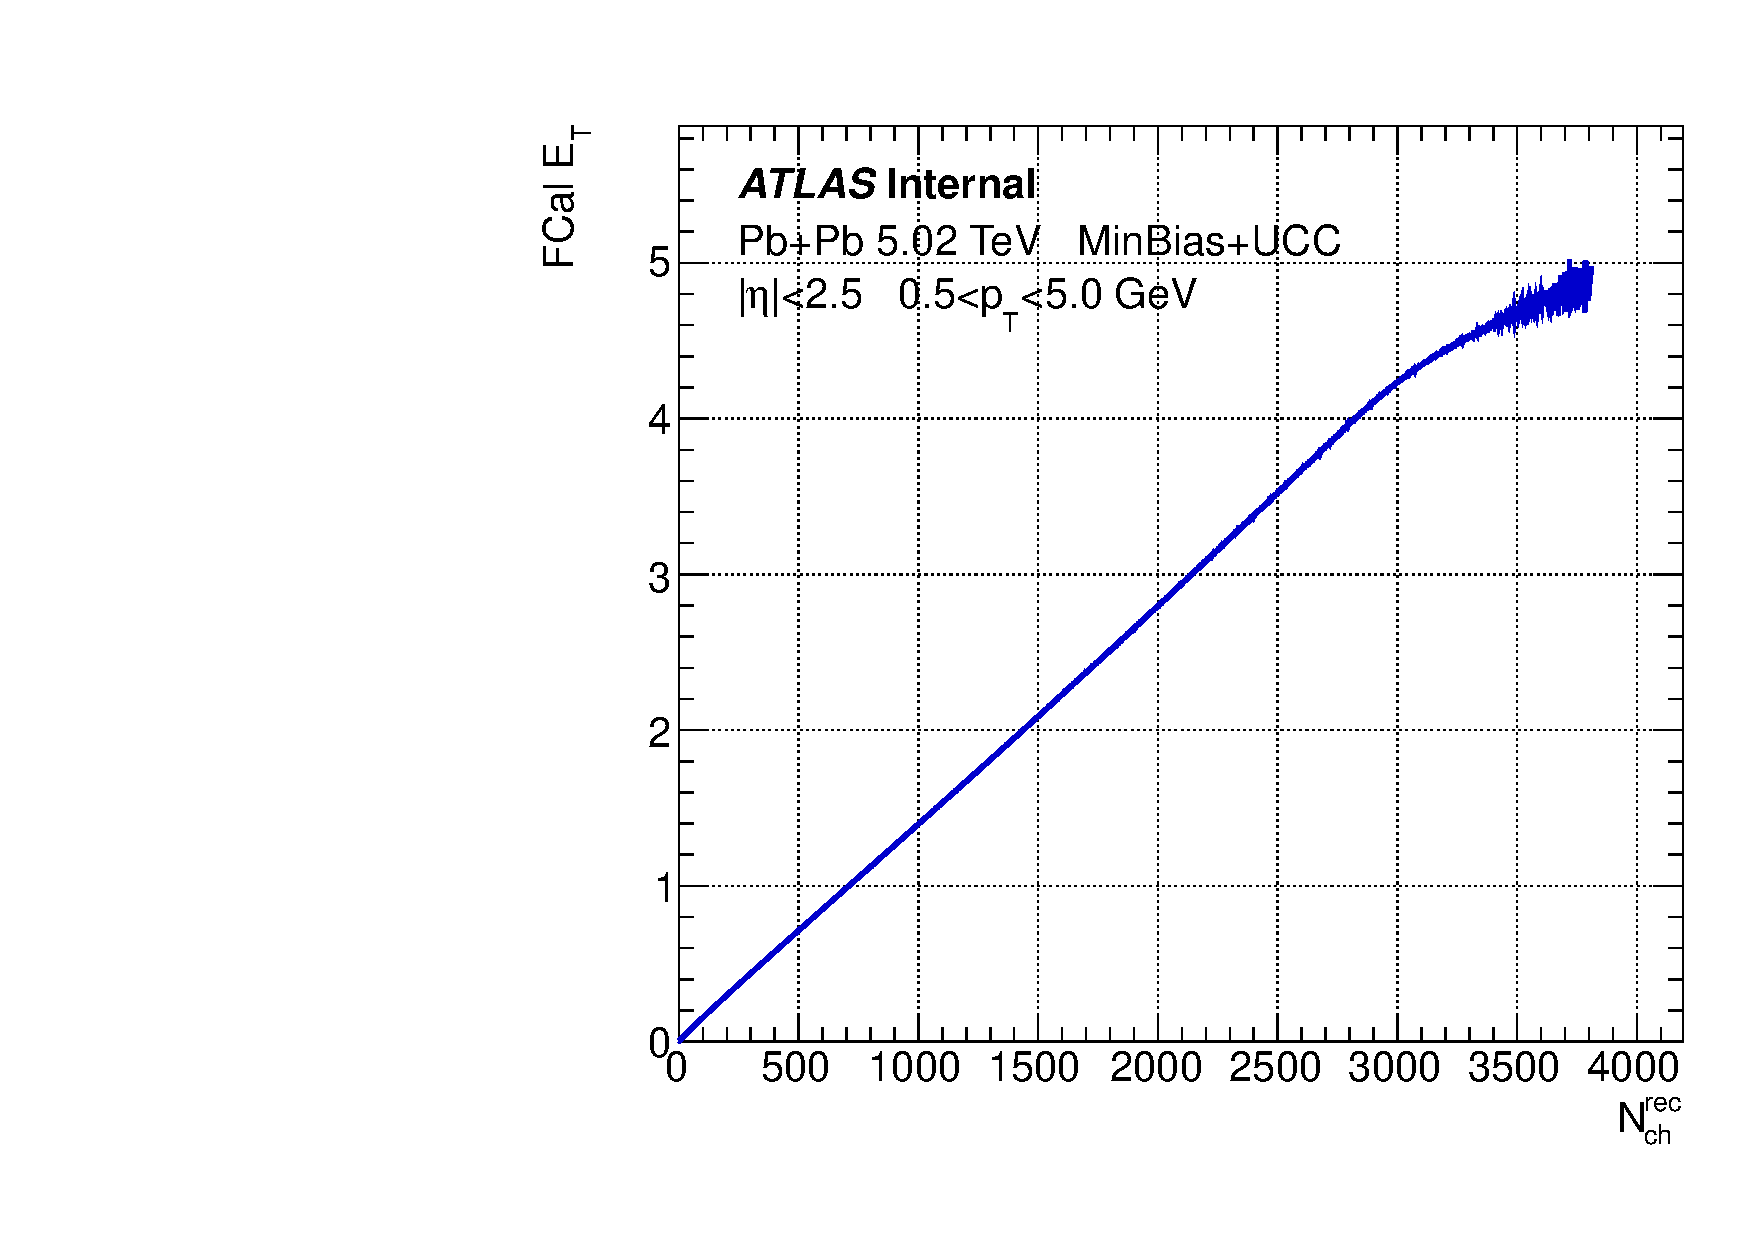
\includegraphics[width=.32\linewidth]{figs/sec_ana/cvtMap_NchRec_fcal.pdf}
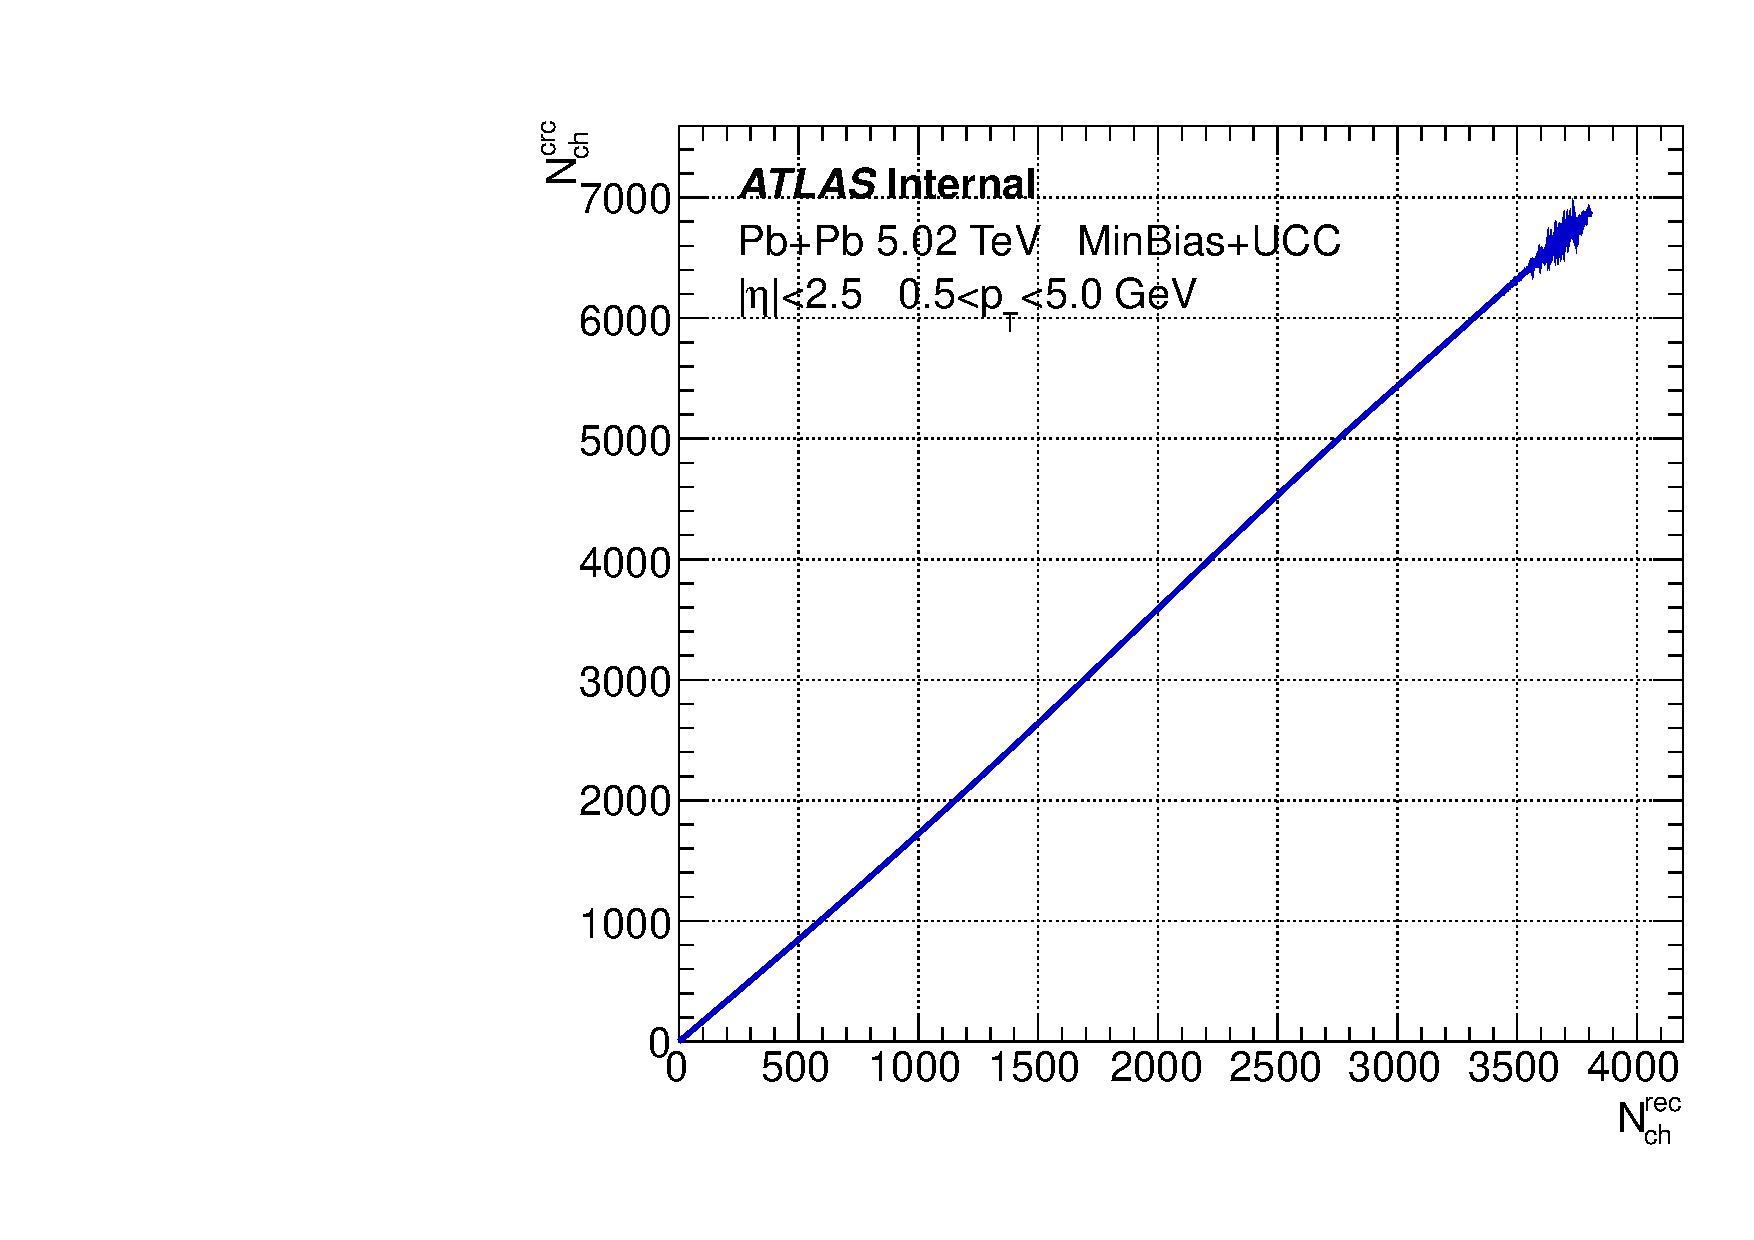
\includegraphics[width=.32\linewidth]{figs/sec_ana/cvtMap_NchRec_NchCrc.pdf}
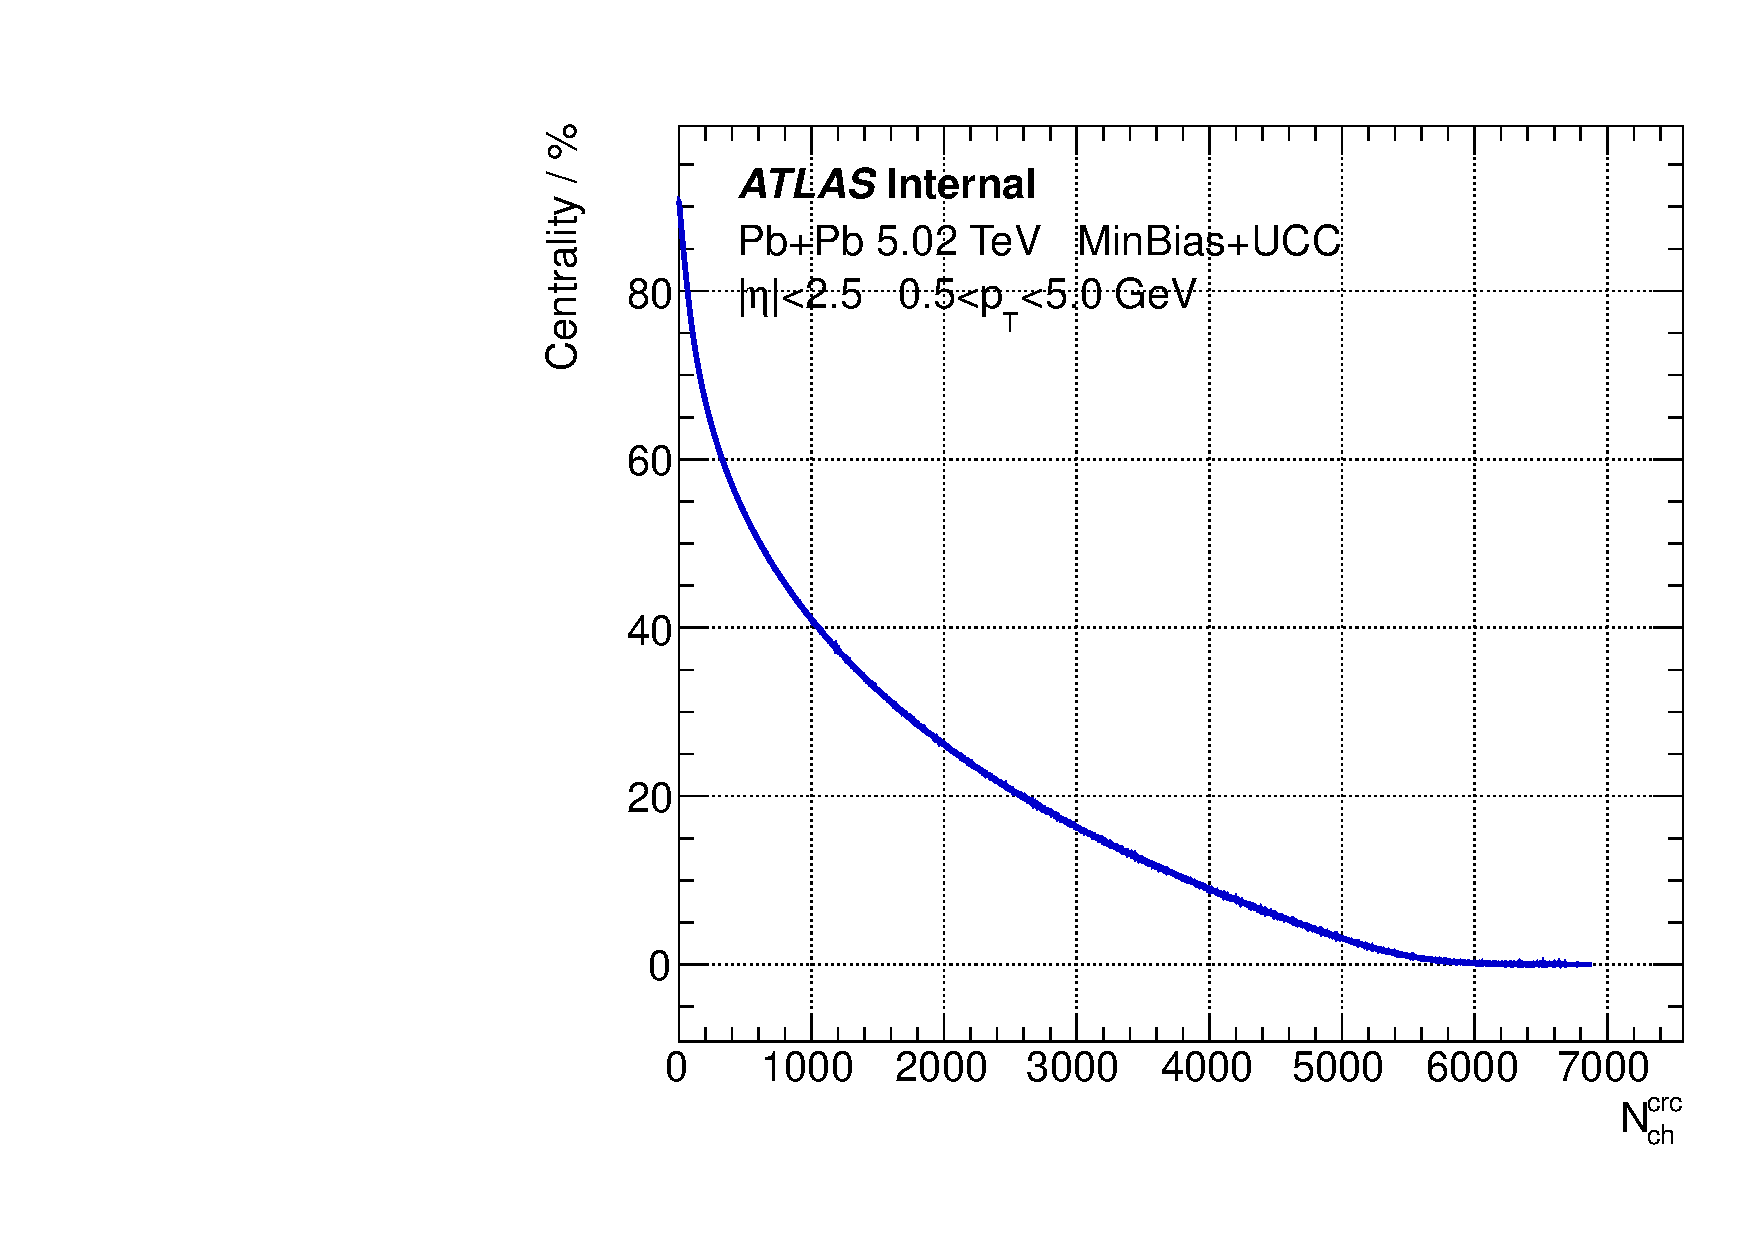
\includegraphics[width=.32\linewidth]{figs/sec_ana/cvtMap_NchCrc_cent.pdf}
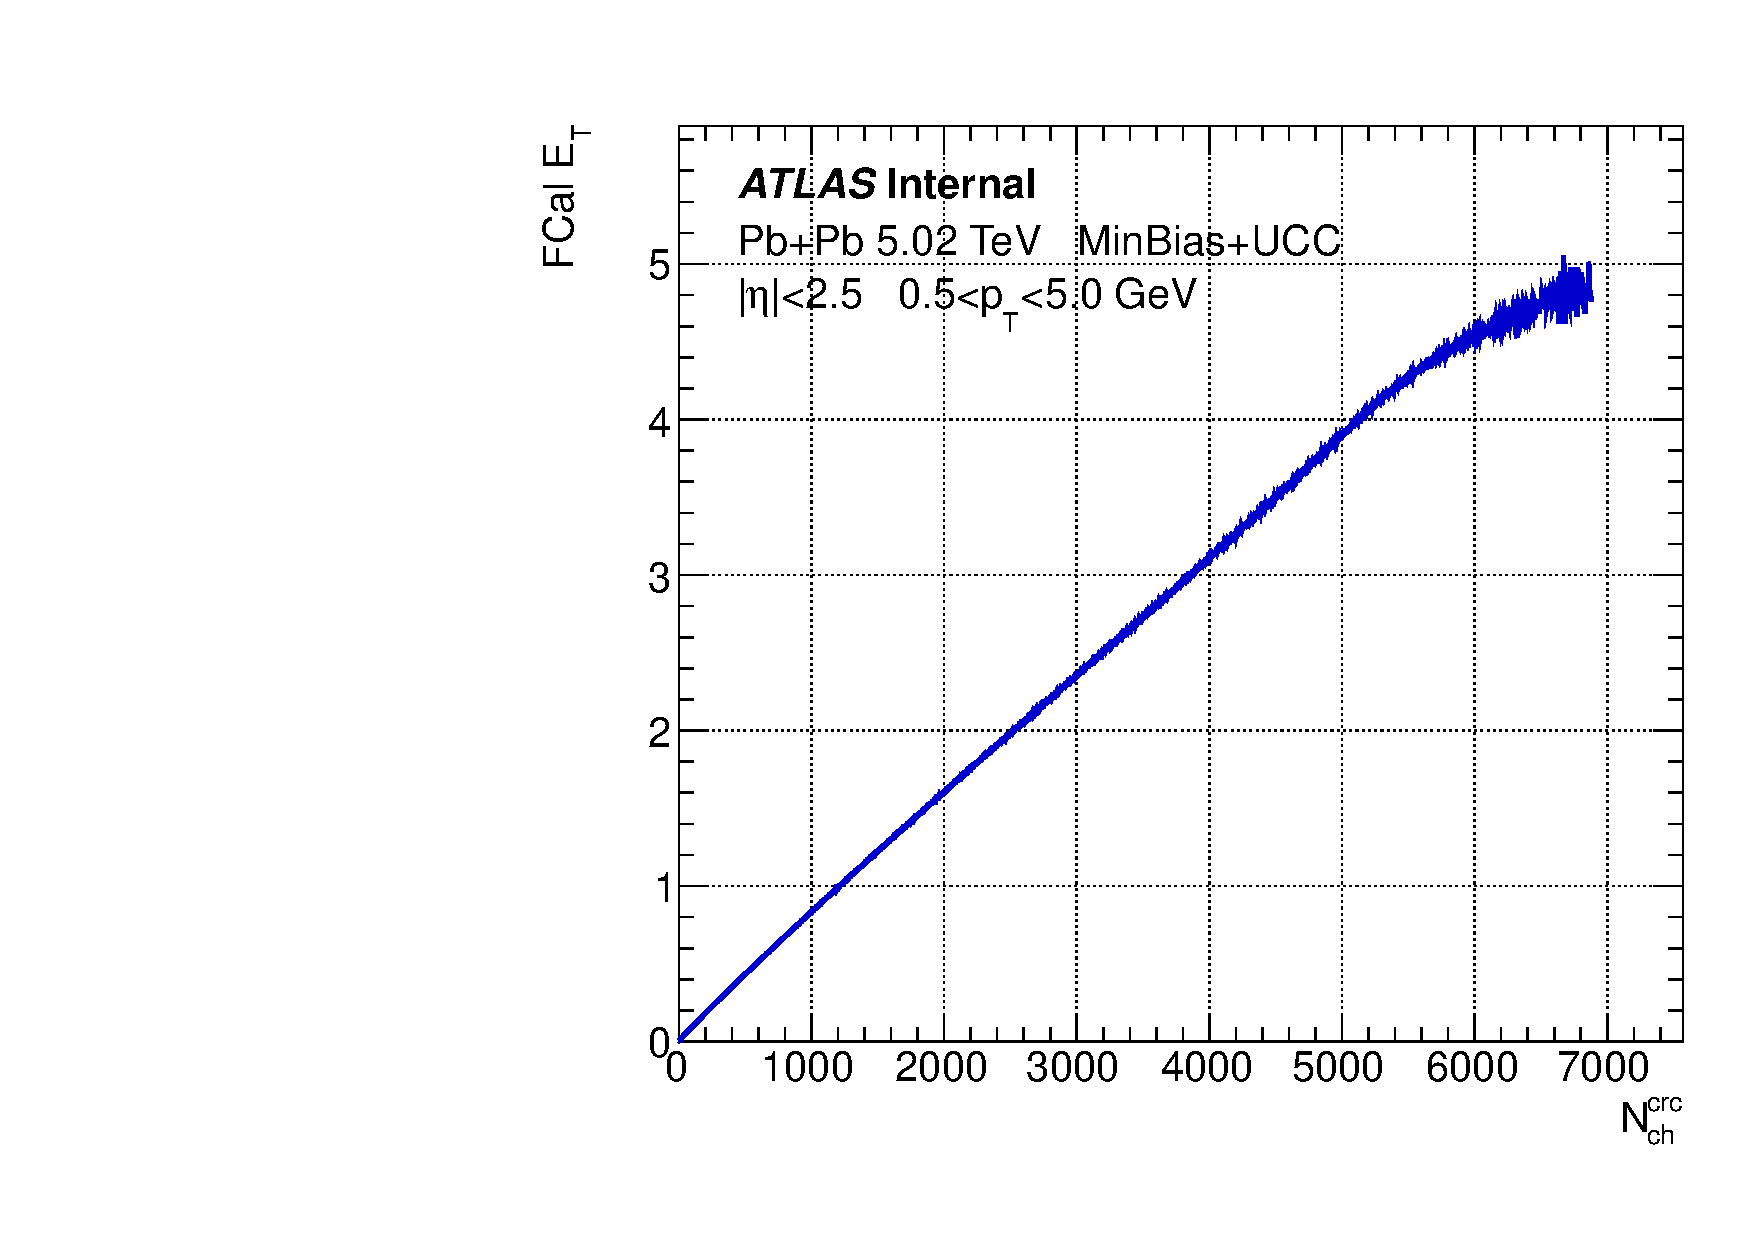
\includegraphics[width=.32\linewidth]{figs/sec_ana/cvtMap_NchCrc_fcal.pdf}
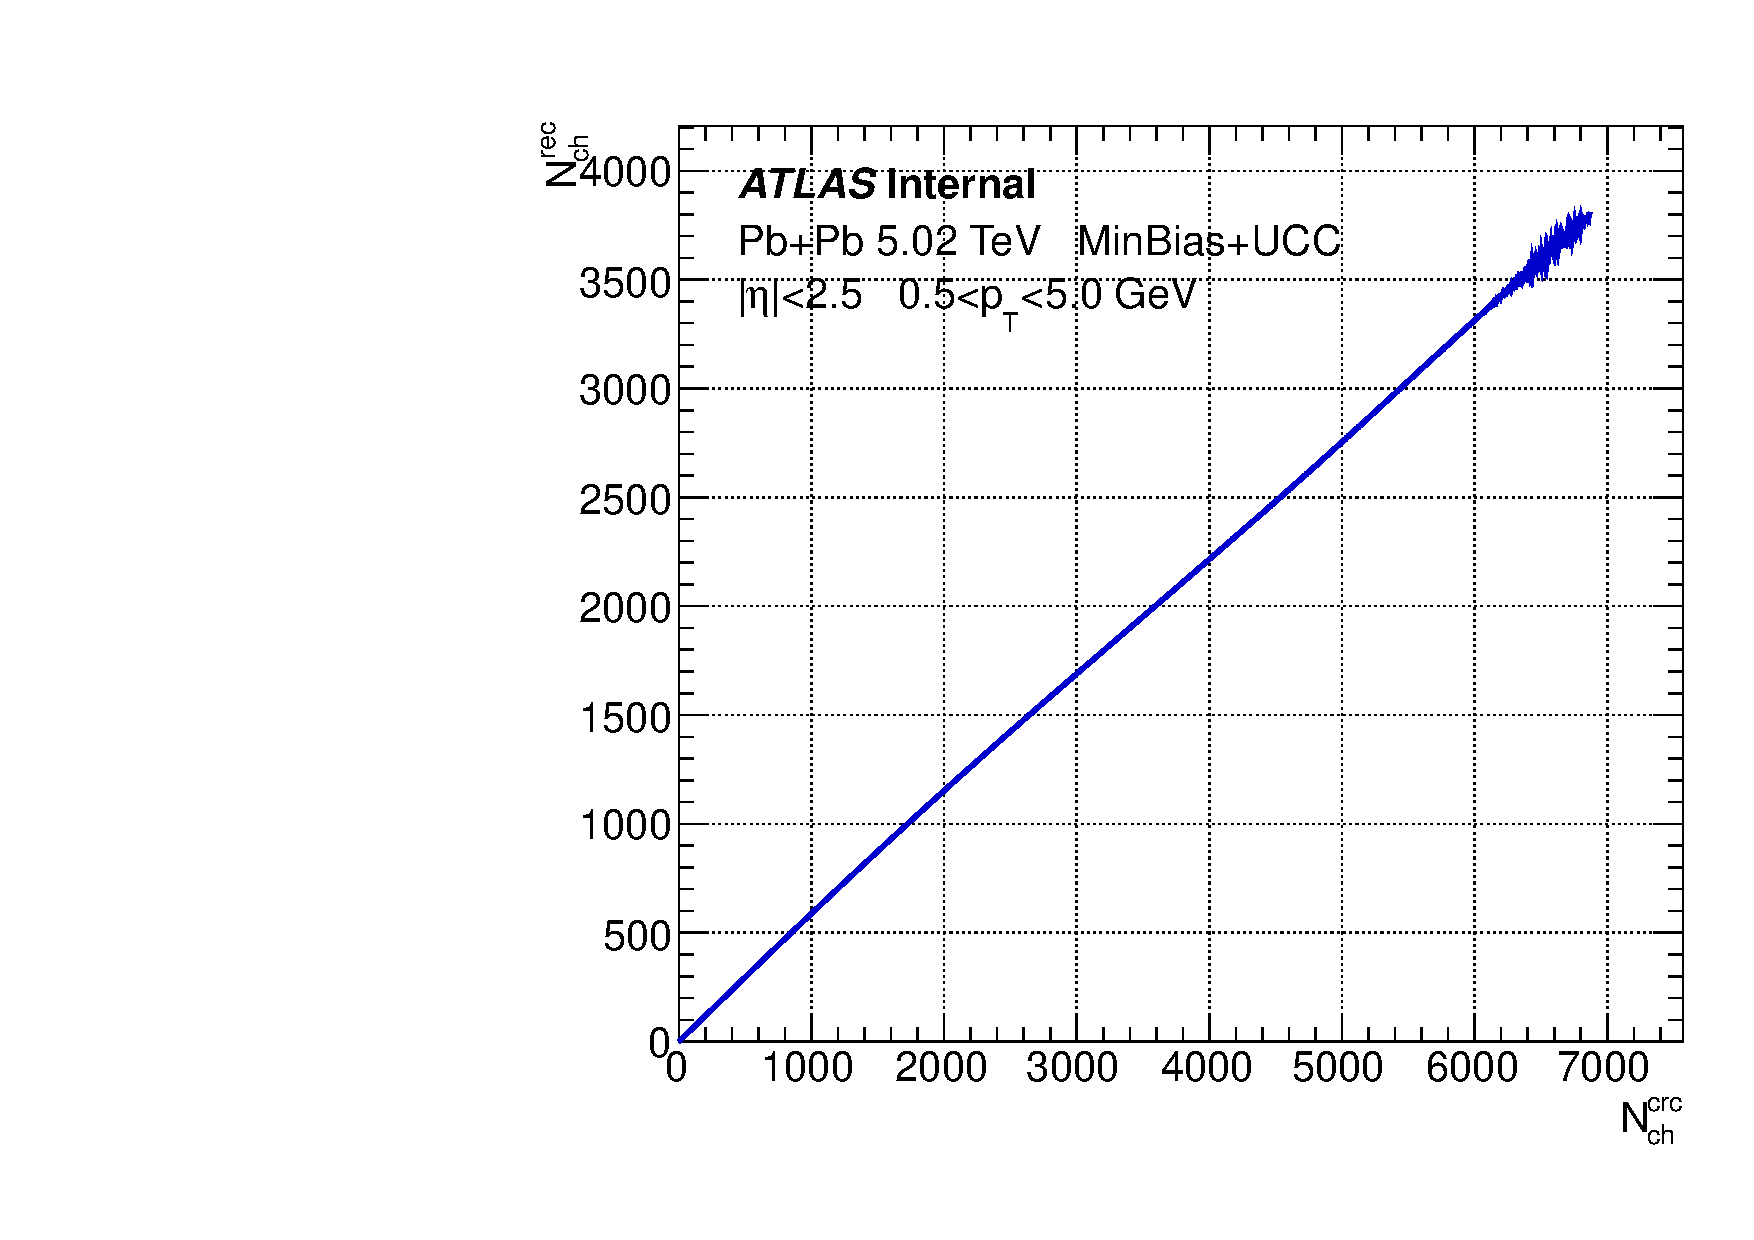
\includegraphics[width=.32\linewidth]{figs/sec_ana/cvtMap_NchCrc_NchRec.pdf}
\caption{Conversion maps among centrality, FCal sum $E_{T}$, reconstructed tracks $N_{ch}^{rec}$ and tracking efficiency corrected reconstructed tracks $N_{ch}^{crc}$. The Y-axis shows the mean value calculated in the event class defined by X-axis.}
\label{fig:ana_cvt}
\end{figure}
The conversion maps among centrality, FCal $E_\text{T}$, number of reconstructed tracks $N_{ch}^{rec}$ and number of corrected reconstructed tracks $N_{ch}^{crc}$ are listed in Fig.~\ref{fig:ana_cvt}, where the Y-axis indicates the mean value calculated in the event class defined by the X-axis. When necessary, these maps are used to convert results with different event class definitions into the same X-axis.



\subsection{Mixed events}
To correct the detector effects, we weighted the tracks by the tracking efficiency and fraction of fake tracks obtained from Monte-Carlo plus the detector simulation. In additional, $w_\phi$ obtained from flattening procedure is applied as the event weight to further suppress the detector effects in the transverse plane. To estimate the residual detector effects, a mixed event technique can be implemented. In this section, we will discuss why mixed event work and how to implement it.

Compared with the physics signal, the major feature of detector effect is that it does not fluctuate from event to event. In other words, detector effects are correlated across "similar" events that are neighbouring in time. By "similar", it requires those events have the similar centrality and $z$ position of primary vertex $z_{vtx}$. On the other hand, the physics signal, like flow, are correlated within a single event, but uncorrelated between different events. Using these features, the mixed event can be reconstructed by measuring the correlation among different events.

In the following we will take the calculation of $c_{n}\{4\}$ as one example to show how to calculate the corresponding mixed events. The definition of 2- and 4-particle correlation in mixed events is written as:
\begin{equation}
\begin{split}
corr_{n}^{bk}\{2\}&\equiv \lr{e^{i\text{n}(\phi_i-\phi_j)}} \\
corr_{n}^{bk}\{4\}&\equiv \lr{e^{i\text{n}(\phi_i+\phi_j-\phi_k-\phi_l)}}
\end{split}
\end{equation}
where $bk$ in the superscript is used to separate the mixed event (background) from the original signal (foreground). The definition seems to be identical to the $corr_{n}\{2k\}$ in a single event, however, now $i, j, k$ and $l$ are particles coming from 4 different events that are neighbouring in time. Note that there are 3 equivalent permutation of $i, j, k$ and $l$: $(\phi_i+\phi_j-\phi_k-\phi_l)$, $(\phi_i+\phi_k-\phi_j-\phi_l)$ and $(\phi_i+\phi_l-\phi_j-\phi_k)$ and they should all be included when calculating the background.

In the definition of $corr_{n}^{bk}\{2\}$ and $corr_{n}^{bk}\{4\}$, since particle can never be correlated with itself, all duplicates are gone. Thus the Q-cumulant formula are much simpler compared with the calculation of foreground:
\begin{equation}
\begin{split}
corr_n^{bk}\{2\}&=\frac{\mathcal{R}\textit{e}(\pmb{Q}_{n,1}^{i}\pmb{Q}_{n,1}^{j*})}{S_{1,1}^i S_{1,1}^j} \\
corr_n^{bk}\{4\}&=\frac{\mathcal{R}\textit{e}(\pmb{Q}_{n,1}^{i}\pmb{Q}_{n,1}^{j}\pmb{Q}_{n,1}^{k*}\pmb{Q}_{n,1}^{l*})}{S_{1,1}^i S_{1,1}^j S_{1,1}^k S_{1,1}^l}
\end{split}
\end{equation}
where $i, j, k$ and $l$ denotes 4 different events.

Then followed the same procedure, the $corr_n^{bk}\{2k\}$ are averaged in each event class to get $\lr{corr_n^{bk}\{2k\}}$. The 4-particle cumulant from background can also be defined in the same way:
\begin{equation}
c_{n}^{bk}\{4\}=\lr{corr_n^{bk}\{4\}}-2\lr{corr_n^{bk}\{2\}}^2
\end{equation}
where the event class is defined by the first event $i$ in the mixed events.

In the end, we subtract the cumulant calculated in mixed events from the foreground, to obtain the corrected cumulant:
\begin{equation}
c_{n}^{crt}\{4\}\equiv c_{n}\{4\}-c_{n}^{bk}\{4\}
\end{equation}
In the measurement section, without special mention, All cumulant results are using $c_{n}^{crt}\{2k\}$ as the default.



\subsection{Statistical uncertainty}
Cumulant analysis, especially for higher order cumulant, suffers from statistics, which makes it crucial to correctly calculated the statistical uncertainty. The errors can be directly calculated from the cumulant definition, by using appropriate error propagation. Take 4-particle standard cumulant as an example:
\begin{equation}
c_n\{4\}=\lr{corr_n\{4\}}-2\lr{corr_n\{2\}}^2
\end{equation}
where both $\lr{corr_n\{4\}}$ and $\lr{corr_n\{2\}}$ are averaged over many events, so the errors are calculated as:
\begin{equation}
\begin{split}
\delta^2(\lr{corr_n\{4\}})&\equiv \frac{\sum_i W^i\{4\}(corr_n^i\{4\}-\lr{corr_n\{4\}})^2}{\sum_i W^i\{4\}} \\
\delta^2(\lr{corr_n\{2\}})&\equiv \frac{\sum_i W^i\{2\}(corr_n^i\{2\}-\lr{corr_n\{2\}})^2}{\sum_i W^i\{2\}}
\end{split}
\end{equation}
However, since the weights $W^i\{4\}$ and $W^i\{2\}$ are not random, there is a correction factor to yield an unbiased estimator:
\begin{equation}
\begin{split}
\delta^2(\lr{corr_n\{4\}})&=(1-\frac{\sum_i (W^i\{4\})^2}{(\sum_i W^i\{4\})^2})\delta^2_\text{real}(\lr{corr_n\{4\}}) \\
\delta^2(\lr{corr_n\{2\}})&=(1-\frac{\sum_i (W^i\{2\})^2}{(\sum_i W^i\{2\})^2})\delta^2_\text{real}(\lr{corr_n\{2\}})
\end{split}
\end{equation}
where $\delta_\text{real}$ means the correct, unbiased statistical error estimator.

Note that both $\lr{corr_n\{4\}}$ and $\lr{corr_n\{2\}}$ measure the flow sign, so they are not independent variables. Thus the covariance needs to be considered while calculating the statistical errors for $c_n\{4\}$:
\begin{equation}
\delta^2(c_n\{4\})=\delta^2_\text{real}(\lr{corr_n\{4\}})+(4\lr{corr_n\{2\}})^2\delta^2_\text{real}(\lr{corr_n\{4\}})-8\lr{corr_n\{2\}}\text{cov}(\lr{corr_n\{4\}},\lr{corr_n\{2\}})
\end{equation}
where the covariance between $\lr{corr_n\{4\}}$ and $\lr{corr_n\{2\}}$ is denoted as $\text{cov}(\lr{corr_n\{4\}},\lr{corr_n\{2\}})$. As can be seen, it is quite cumbersome to calculate statistical error in this way: many histograms need to be saved in order to calculate the covariance. Furthermore, the formula are more complicated in subevent methods: up to 10 covariances will show up in the formula! Due to this reason, in this analysis, sub-sample technique is used to determine the statistical errors.

The sub-sample technique is a data-driven way to calculate the statistical errors, which is much easier to implement in the code. The first step is to randomly divide the whole data set into $N$ sub-samples ($N=20$ in this analysis). To guarantee that each sub-sample are not biased by run configuration like trigger setup and detector effects, in practice, we used random seeds to determine which sub-sample each event will fall into, which guarantees the dividing procedure to be random.

To demonstrate the random seed works, we have tested this produce on the 2015+2016 13 TeV low-$\mu$ $pp$ sample. The reason of choosing $pp$ is because the runs are throughout two years and run conditions as well as trigger setups are very different. The results are presented in Fig.~\ref{fig:ana_div}. Left plot shows the $N_{ch}$ distribution for the whole sample, where several "bumps" are from the high-multiplicity track (HMT) triggers. Right plot shows the relative difference of the statistics between sub-samples (indicated by different colors) and the mean ($5\%$ statistics of the whole sample), as a function of $N_{ch}$. As can be seen, the relative difference is within $1\%$ in the region where statistics are good. This demonstrates the dividing procedure produces randomly divided sub-samples.
\begin{figure}[H]
\centering
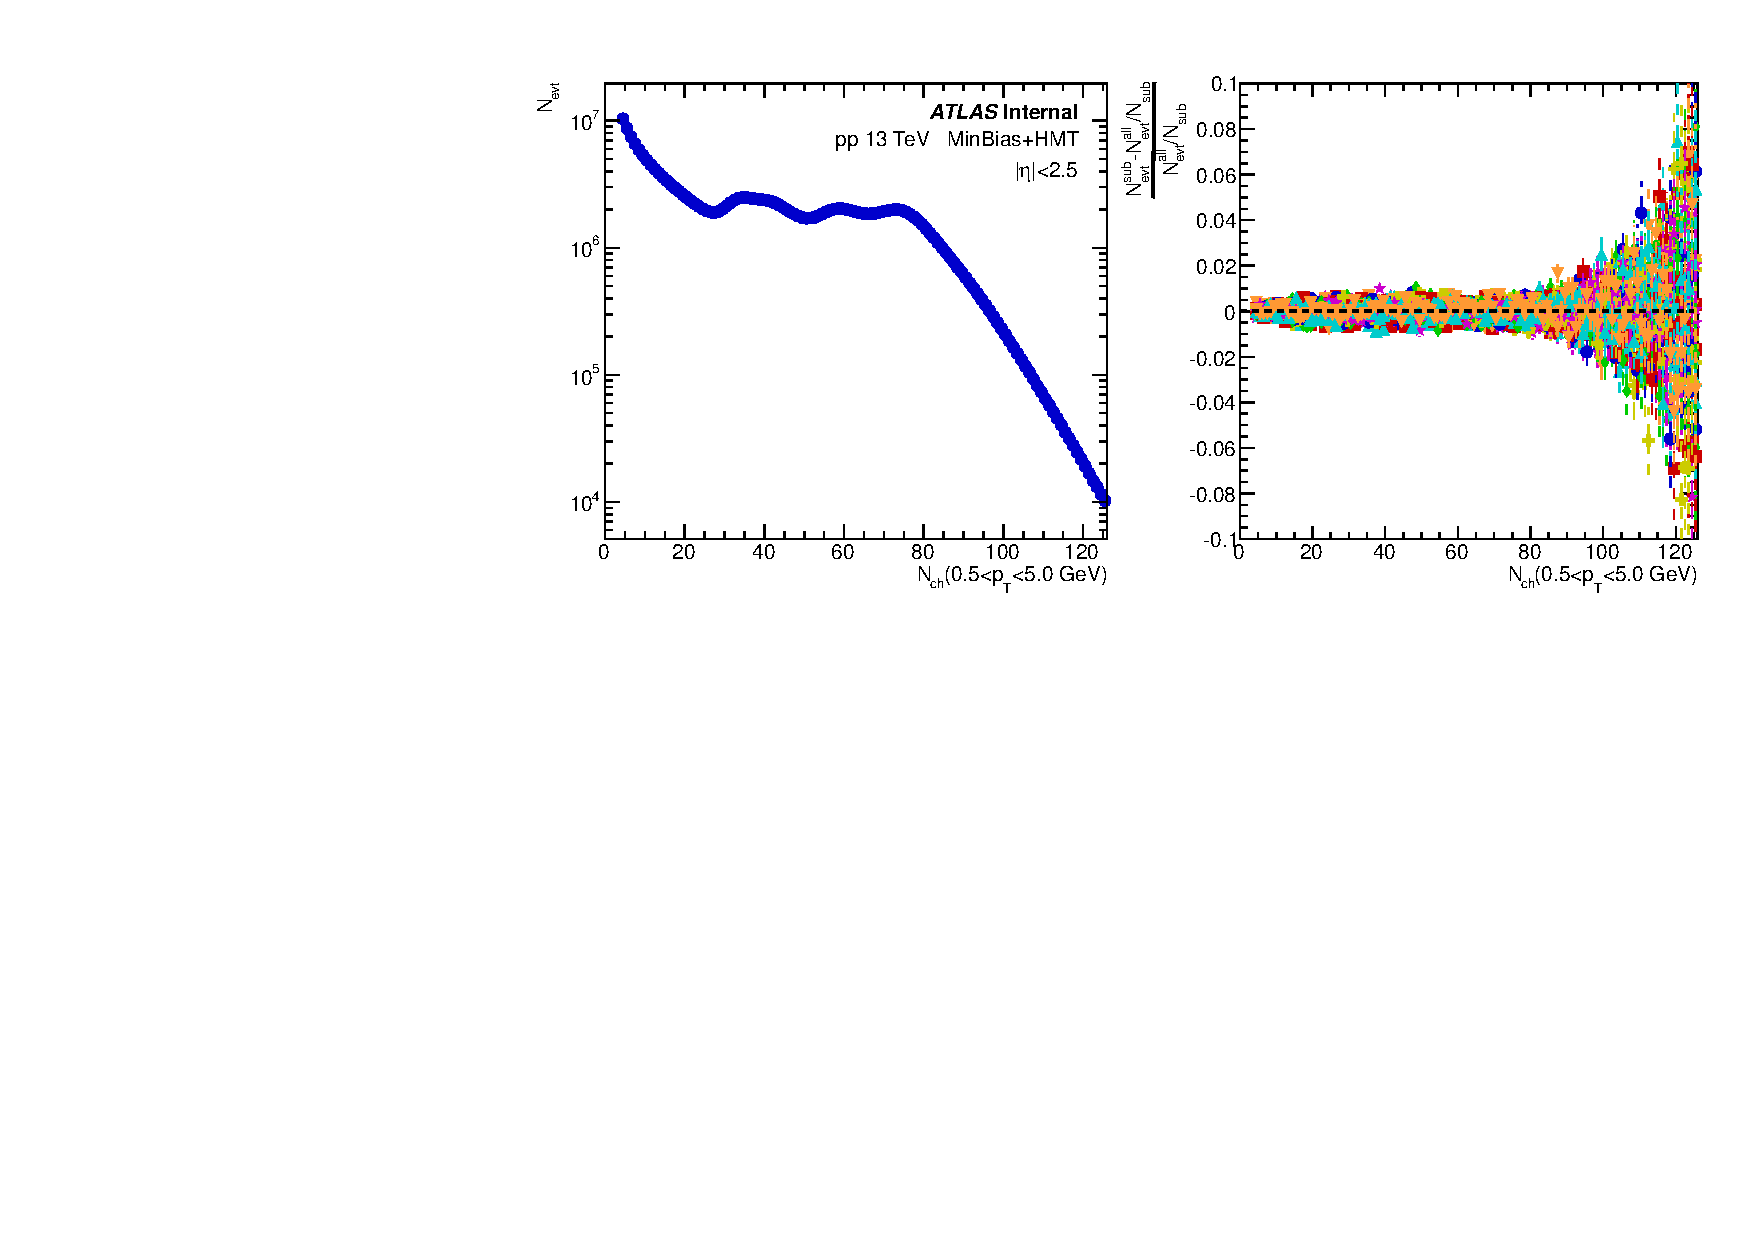
\includegraphics[width=.9\linewidth]{figs/sec_ana/pp13_chk_division.pdf}
\caption{$N_{ch}$ distribution for the whole 13 TeV $pp$ data sample (left); Right plot shows the relative difference of the statistics between sub-samples (indicated by different markers and colors) and the mean ($5\%$ statistics of the whole sample). The results are shown as a function of $N_{ch}$.}
\label{fig:ana_div}
\end{figure}

Then the $2k$-particle cumulant are calculated in whole sample, as well as in each sub-sample respectively. The standard deviation of cumulants calculated from all sub-samples are quoted as the statistical uncertainty of the cumulant for the whole sample.


